% Tesi Informatica Bicocca - Cristiano Rotunno 914317

% Carattere dimensione 12
\documentclass[12pt]{report}

% Per la stampa fronte-retro sostituire con:
%\documentclass[12pt, twoside]{report}

% Margini (4cm a sx, 2.5cm a dx, 2.5cm in alto, 2.5cm in basso)
\usepackage[top=2.5cm, bottom=2.5cm, left=4cm, right=2.5cm, centering, head=21.75 pt]{geometry}

% Interlinea standard 1.5
\linespread{1.5}

% --- Pacchetti Fondamentali per Lingua e Font ---
\usepackage[T1]{fontenc}      % Gestione corretta dei caratteri accentati (evita buchi nel testo)
\usepackage[utf8]{inputenc}    % Codifica caratteri
\usepackage[italian]{babel}    % Sillabazione italiana
\usepackage{microtype}         % MIGLIORA LA GIUSTIFICAZIONE: risolve i problemi di spaziature eccessive
\usepackage{mathptmx}         % Font simile al Times New Roman

% --- Librerie Matematiche e Grafiche ---
\usepackage{amsmath} 
\usepackage{amsthm} 
\usepackage{amssymb}
\usepackage{graphicx} 
\usepackage{subfigure}
\usepackage{booktabs}
\usepackage{caption}
\usepackage{float} 

% --- Gestione Pagina e Stili ---
\usepackage{scrlayer-scrpage} 
\usepackage{parskip}
\ifoot[]{}
\cfoot[]{}
\ofoot[\pagemark]{\pagemark}
\pagestyle{scrplain}

% --- Bibliografia e Citazioni ---
\usepackage{csquotes} 
\usepackage[backend=biber, sorting=nty]{biblatex} 
\usepackage[hidelinks]{hyperref}
\usepackage{url}
\appto{\bibsetup}{\raggedright}
\addbibresource{bibliography.bib}

% --- Formattazione Titoli ---
\usepackage{titlesec} 
\titleformat{\chapter}[block]
  {\normalfont\LARGE\bfseries}{\thechapter.}{0.5em}{\LARGE}
\titlespacing*{\chapter}{0pt}{-20pt}{25pt}

% --- Gestione Codice Sorgente (HLSL/C#) ---
\usepackage{xcolor}
\usepackage{listings}

% Definizione Colori Soft/Professional
\definecolor{code_bg}{RGB}{245,245,247}      % Grigio chiarissimo (stile Apple/GitHub)
\definecolor{code_keyword}{RGB}{0,51,153}    % Blu scuro professionale
\definecolor{code_comment}{RGB}{120,120,120} % Grigio medio per i commenti
\definecolor{code_string}{RGB}{163,21,21}    % Rosso scuro per le stringhe
\definecolor{code_text}{RGB}{30,30,30}       % Testo quasi nero
\definecolor{code_func}{RGB}{102,0,153}      % Viola per le funzioni

\lstdefinelanguage{pseudo}{
    morekeywords={for, each, in, if, else, return, new, function, while, break},
    sensitive=false,
    morecomment=[l]{//},
    morecomment=[s]{/*}{*/},
    morestring=[b]",
}

\lstset{
    language=pseudo,
    backgroundcolor=\color{code_bg},
    basicstyle=\color{code_text}\ttfamily\small,
    keywordstyle=\color{code_keyword}\bfseries,
    commentstyle=\color{code_comment}\itshape,
    stringstyle=\color{code_string},
    % Definizione funzioni per evidenziarle nel testo
    emph={Draw, FindStaticObjectsWith, TransformToWorldSpace, AddVertices, BindMesh, BindMaterial, UploadToCBuffer, DrawInstanced},
    emphstyle=\color{code_func},
    % Layout pulito
    numbers=none,           % Tolti i numeri di riga
    frame=none,             % Tolte le linee di bordo
    showspaces=false,
    showstringspaces=false,
    breaklines=true,
    tabsize=4,
    xleftmargin=10pt,       % Piccolo rientro per staccarlo dal testo
    xrightmargin=10pt,
    aboveskip=15pt,         % Spazio prima del codice
    belowskip=15pt          % Spazio dopo il codice
}

\includeonly{capitolo1}

\begin{document}

% Frontespizio
\begin{titlepage}
\begin{center}
    {\LARGE{Università degli Studi di Milano Bicocca \\}}
    {\small{Dipartimento di Informatica, Sistemistica e Comunicazione}}\\
    {\small{Corso di Laurea Triennale}}
\end{center}
    
\begin{figure}[H]
    \centering
    
\includegraphics[width=0.4\textwidth]{logo.png}
\end{figure}

\begin{center}
    {\Large { Analisi e ottimizzazione del videogioco Ares tramite tecniche di rendering in Unity }}
\end{center}

\vspace{2cm}

\begin{minipage}[t]{0.47\textwidth}
	{\large{\bf Relatore:\\ Prof. Gianluigi Ciocca}}
	\vspace{0.5cm}
	{\large{\bf \\Correlatore:\\ Dott. Davide Marelli}}
\end{minipage}\hfill\begin{minipage}[t]{0.47\textwidth}\raggedleft
	{\large{\bf Candidato: \\Cristiano Rotunno\\ }}
\end{minipage}

\vspace{25mm}

\centering{\large{\bf ANNO ACCADEMICO 2025/2026 }}
\end{titlepage}
% Fine frontespizio

\tableofcontents
\thispagestyle{empty}

% --- Struttura Capitoli ---

% Introduzione
\addcontentsline{toc}{chapter}{Introduzione} 
\chapter*{Introduzione}

L'industria dello sviluppo di videogiochi ha raggiunto negli ultimi anni livelli di complessità tecnica e fedeltà visiva senza precedenti. In questo contesto, l'utilizzo di motori grafici avanzati come Unity permette di realizzare scenari fotorealistici, ma pone sfide significative in termini di efficienza computazionale e gestione delle risorse hardware.

\begin{figure}[htbp]
    \centering
    \begin{minipage}{0.48\textwidth}
        \centering
        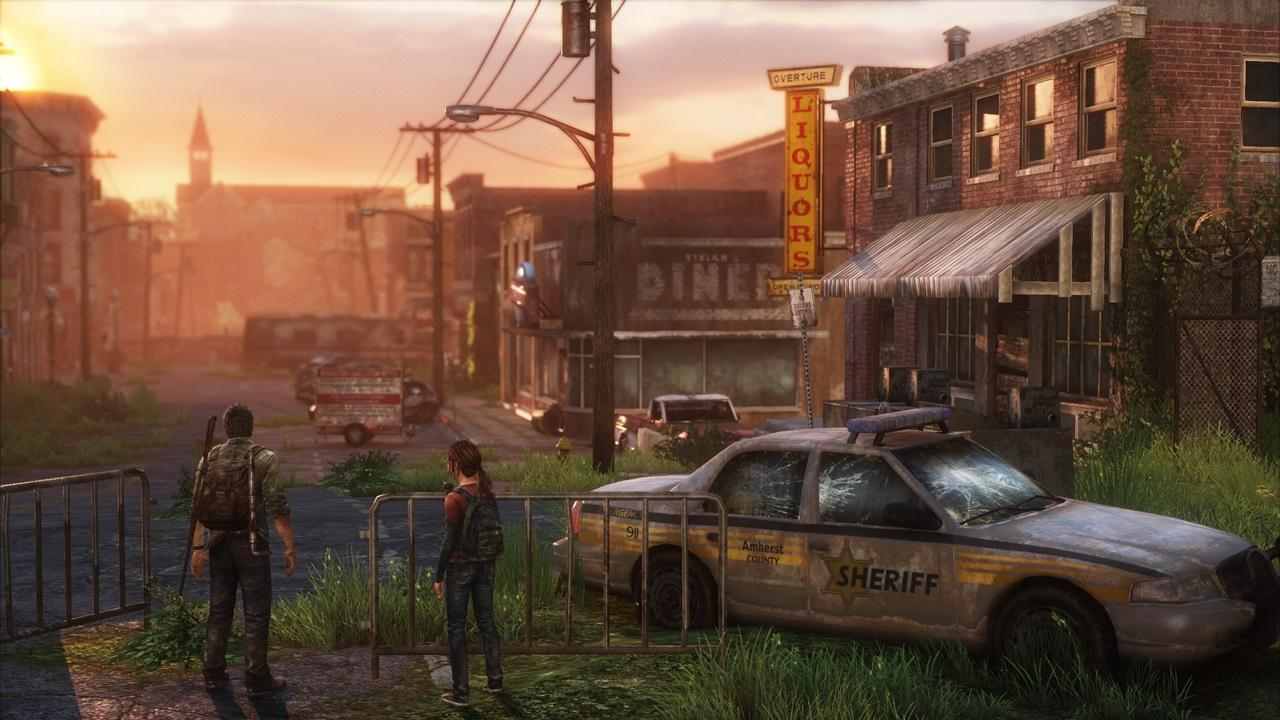
\includegraphics[width=\textwidth]{immagini/lastofus.jpg}
        \caption*{\small The Last Of Us.}
    \end{minipage}
    \hfill % Spazio flessibile tra le due immagini
    \begin{minipage}{0.48\textwidth}
        \centering
        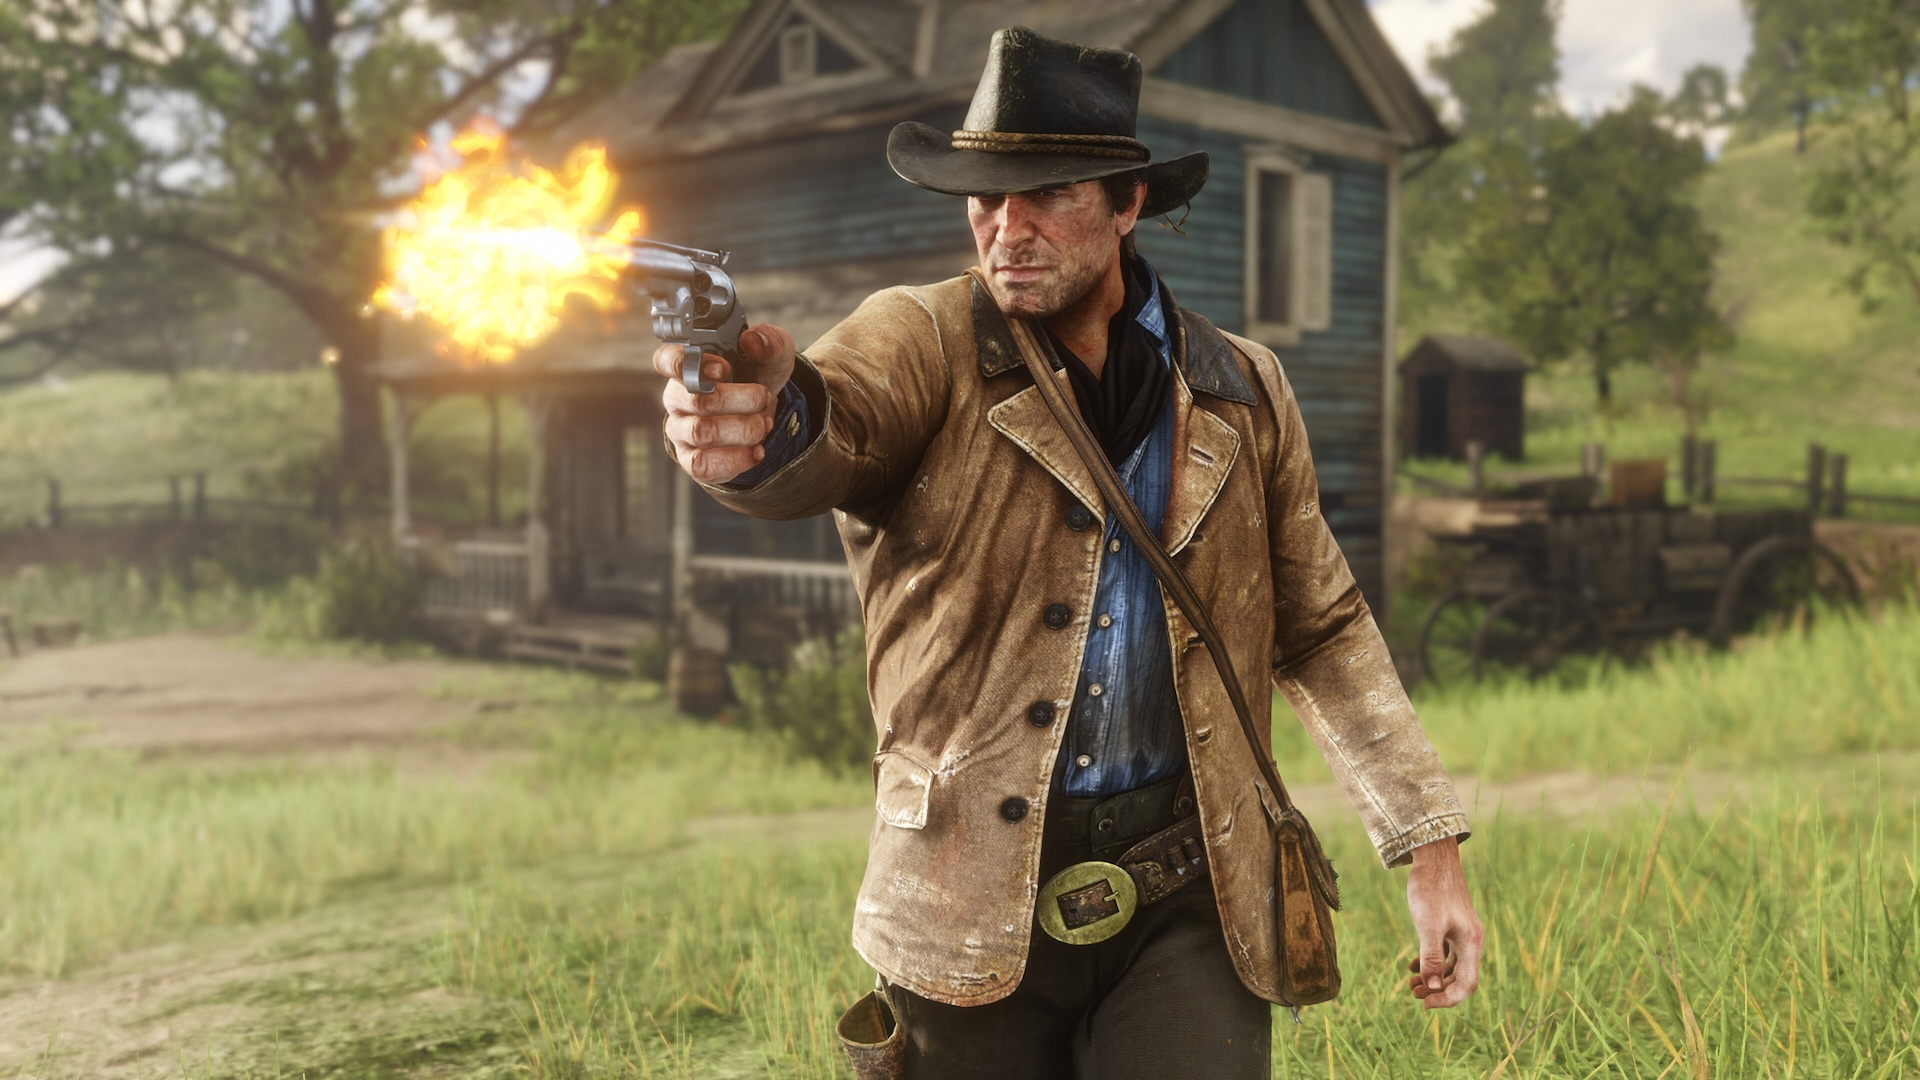
\includegraphics[width=\textwidth]{immagini/rdr2.jpg}
        \caption*{\small Red Dead Redemption II}
    \end{minipage}
\end{figure}

Il progetto, denominato ARES, consiste in un videogioco sviluppato tramite la High Definition Rendering Pipeline (HDRP) di Unity, una tecnologia progettata per massimizzare la resa grafica a fronte di un elevato carico sulla GPU. L'obiettivo principale della sperimentazione è stato l'analisi e l'ottimizzazione delle performance di rendering del titolo. In particolare, l'attenzione si è focalizzata sulla riduzione delle \textit{draw call}, sulla gestione dei \textit{batch} e sullo sviluppo di shader personalizzati volti a migliorare il frame rate senza compromettere la qualità estetica. % Crea il file introduzione.tex

\clearpage

% Capitolo 1: Ares
\chapter{Il Progetto ARES}
\section{Presentazione del videogioco ARES}
Il progetto ARES consiste nello sviluppo di un videogioco appartenente al genere \textit{First-Person Shooter} (FPS), progettato per una distribuzione multipiattaforma su sistemi operativi macOS e Microsoft Windows. L'opera si prefigge l'obiettivo di raggiungere standard qualitativi paragonabili alle produzioni di fascia "AAA", puntando su un'elevata fedeltà visiva e su un'immersività garantita da scenari complessi e dettagliati.

Dal punto di vista tecnico, il software è stato realizzato utilizzando il motore grafico Unity, avvalendosi specificamente della \textit{High Definition Rendering Pipeline} (HDRP). Questa scelta è stata dettata dalla necessità di gestire sistemi di illuminazione avanzata di tipo \textit{Mixed} (combinazione di luci in tempo reale e pre-calcolate) e materiali ad alta risoluzione, fondamentali per caratterizzare le diverse ambientazioni di gioco, che spaziano da complessi industriali a quartieri urbani densamente popolati.

\begin{figure}[htbp]
    \centering
    \begin{minipage}{0.48\textwidth}
        \centering
        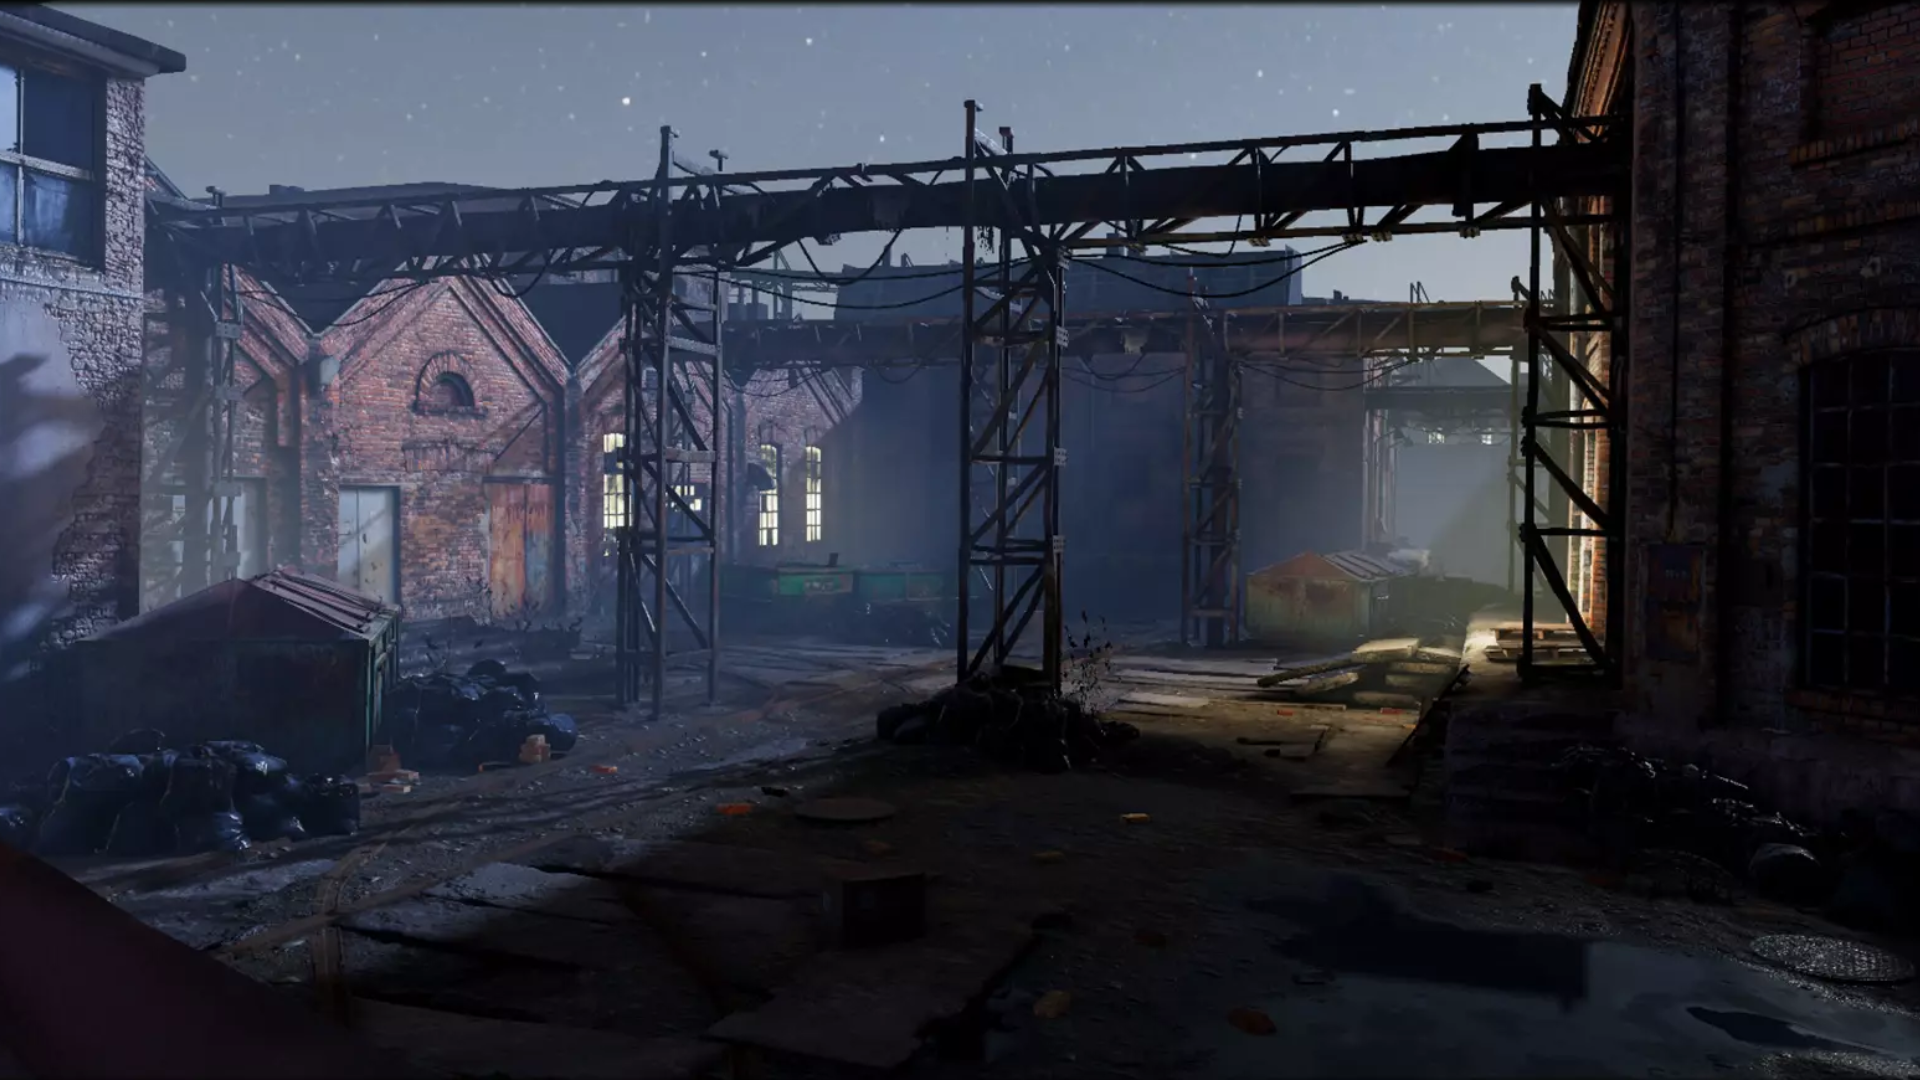
\includegraphics[width=\textwidth]{immagini/map_urban.png}
    \end{minipage}
    \hfill % Spazio flessibile tra le due immagini
    \begin{minipage}{0.48\textwidth}
        \centering
        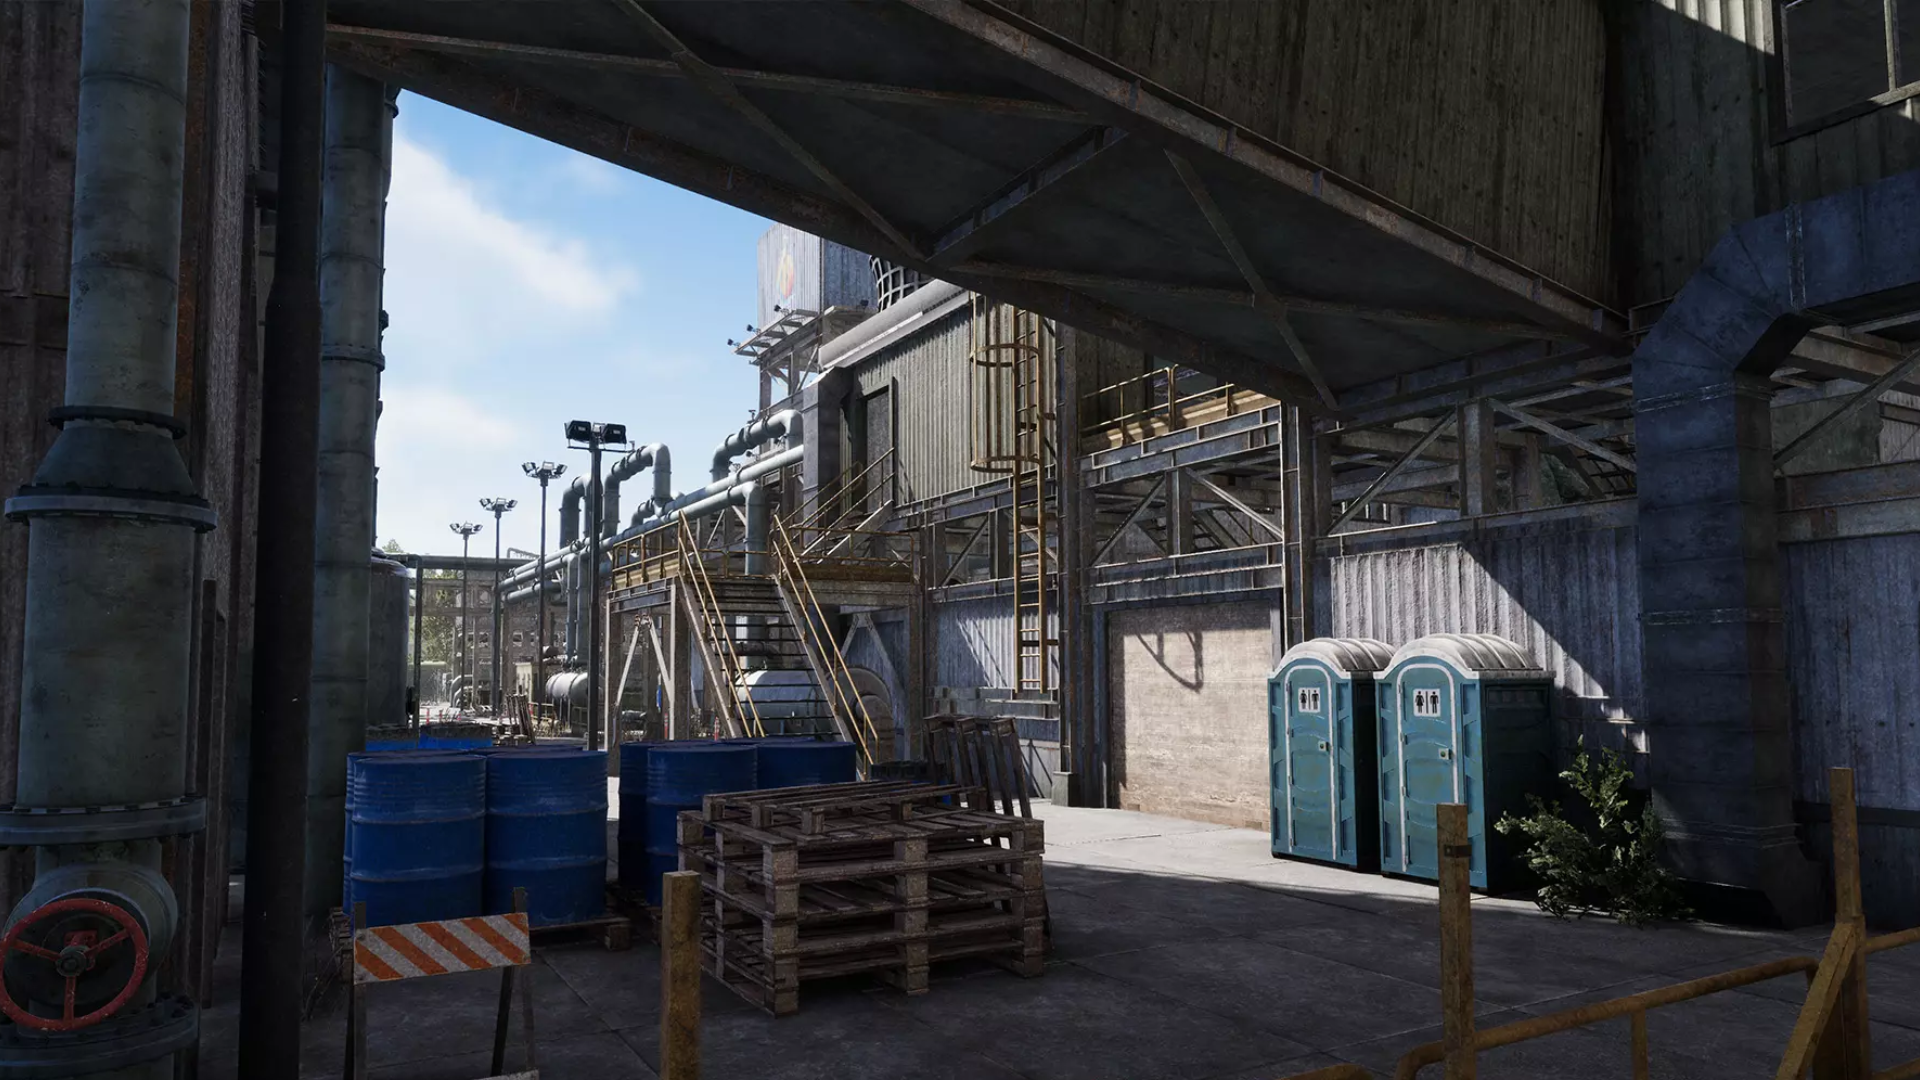
\includegraphics[width=\textwidth]{immagini/map_chemical.png}
    \end{minipage}
    
\end{figure}

Attualmente, il progetto si presenta in una fase di sviluppo avanzata e funzionalmente completa: le meccaniche di base del \textit{gameplay} risultano interamente implementate e il titolo è pienamente giocabile. Nonostante le prestazioni rilevate sulla piattaforma di test (Apple M2 Pro) si attestino su valori ottimali di circa 60 FPS con impostazioni grafiche massime, la vastità delle mappe e l'elevato numero di vertici da renderizzare pongono sfide significative per l'hardware meno performante.

Lo stage si inserisce dunque in questa fase critica del ciclo di vita del software, con l'obiettivo di rifinire la gestione delle risorse grafiche e preparare il motore di gioco per l'introduzione dei contenuti finali e il successivo rilascio. 

Maggiori informazioni sono reperibili presso il sito ufficiale: \\ \url{https://aresofficial.net}.

\section{Motivazioni e obiettivi}
L'attuale mercato dei videogiochi \textit{First-Person Shooter} risulta estremamente competitivo e caratterizzato da standard tecnici elevatissimi. In questo scenario, il progetto ARES nasce con una forte impronta strategica rivolta all'ecosistema macOS, una piattaforma storicamente meno presidiata dai titoli FPS di fascia alta, con l'intento di offrire agli utenti Apple un'esperienza di gioco di qualità comparabile alle produzioni Windows.

Tuttavia, l'obiettivo centrale del presente lavoro di tesi trascende la specifica piattaforma di riferimento, focalizzandosi sull'ottimizzazione trasversale delle prestazioni grafiche su tutti i sistemi operativi supportati. Indipendentemente dall'hardware utilizzato, la fluidità di gioco rappresenta il fattore critico per garantire un'esperienza utente soddisfacente in un titolo competitivo. La ricerca si pone dunque il compito di individuare un \textit{trade-off} ottimale tra fedeltà visiva e velocità di calcolo, massimizzando l'efficienza della pipeline di rendering HDRP per garantire stabilità e alte prestazioni su un'ampia gamma di configurazioni hardware.

Nello specifico, si prefiggono i seguenti obiettivi tecnici e formativi:
\begin{itemize}
\item \textbf{Analisi delle prestazioni:} utilizzo avanzato dello \textit{Unity Profiler} per identificare i \textit{bottleneck} del sistema e comprendere l'impatto dei processi sulla GPU e sulla CPU.
\item \textbf{Ottimizzazione degli Shader:} revisione degli shader esistenti e sviluppo di nuove soluzioni \textit{custom} per ridurre il carico computazionale senza sacrificare il dettaglio grafico.
\item \textbf{Efficienza geometrica:} studio di tecniche per sostituire, ove possibile, istanze di oggetti 3D complessi con shader specifici, riducendo drasticamente il numero di poligoni e di \textit{draw call} inviate al processore grafico.
\item \textbf{Stabilità del Frame Rate:} garantire che l'ottimizzazione porti non solo a un incremento degli FPS medi, ma soprattutto a una stabilità costante del flusso video per evitare fenomeni di \textit{stuttering} durante le sessioni di gioco più concitate.
\end{itemize} % Contenuto: 1.1 Presentazione, 1.2 Motivazioni

\clearpage

% Capitolo 2: Pipeline
\chapter{La Pipeline di Rendering in Unity}

\section{Introduzione a HDRP}

La \textit{High Definition Render Pipeline} (HDRP) rappresenta l'approccio moderno di Unity per la gestione del rendering ad alta fedeltà, progettato specificamente per piattaforme hardware di fascia alta \cite{UnityHDRP}. A differenza della precedente \textit{Built-in Render Pipeline}, la HDRP non è un sistema statico, ma costituisce un'implementazione avanzata della \textit{Scriptable Render Pipeline} (SRP). 

L'architettura SRP introduce un cambio di paradigma fondamentale: il loop di rendering non è più codificato rigidamente all'interno del motore grafico, ma viene esposto tramite un'API C\#. Questo permette agli sviluppatori di estendere, modificare e ottimizzare il processo di disegno dei fotogrammi in base alle esigenze specifiche del progetto, un requisito essenziale per un lavoro di ottimizzazione mirato come quello richiesto da ARES \cite{GregoryGameEngine}.

Il pilastro filosofico della HDRP è il \textit{Physically Based Rendering} (PBR), un modello che mira a simulare l'interazione della luce con le superfici seguendo le leggi della fisica ottica \cite{PharrPBRT}. Per garantire tale coerenza, la pipeline opera esclusivamente in spazio colore lineare e utilizza calcoli in virgola mobile a 32 bit (FP32) \cite{AkenineRealTimeRendering}. Questo garantisce una gamma dinamica elevata (\textit{High Dynamic Range}), permettendo una gestione accurata di contrasti luminosi estremi e materiali complessi, ma introducendo al contempo un carico computazionale significativo che necessita di strategie di gestione della memoria e della GPU estremamente oculate.


\section{Gestione del carico computazionale}

Nel campo della computer grafica in tempo reale, la generazione di un fotogramma non dipende esclusivamente dalla potenza di calcolo della GPU, ma è il risultato di una complessa coordinazione tra quest'ultima e la CPU. Uno dei principali fattori che influenzano le prestazioni di un motore grafico come Unity è il numero di \textit{draw call} effettuate per ogni \textit{frame}.

\subsection{Il costo delle Draw Call}

Una \textit{draw call} può essere definita come un comando inviato dalla CPU alla GPU attraverso un'API grafica per istruire il processore grafico sul disegno di un determinato oggetto o di una porzione di geometria \cite{AkenineRealTimeRendering}. Sebbene la GPU sia estremamente efficiente nel processare migliaia di poligoni in parallelo, la preparazione di ogni singolo comando di disegno comporta un costo significativo per la CPU, noto come \textit{overhead} del driver \cite{GregoryGameEngine}.

Ogni volta che viene invocata una \textit{draw call}, il processore deve eseguire diverse operazioni preliminari:
\begin{itemize}
    \item Verificare lo stato della \textit{pipeline} di rendering.
    \item Impostare i parametri corretti all'interno della memoria della GPU.
    \item Tradurre i comandi del motore grafico in istruzioni comprensibili dal driver hardware.
\end{itemize}

Quando il numero di questi comandi è eccessivo, la CPU non riesce a prepararli con una velocità sufficiente a mantenere il \textit{frame rate} target, portando il sistema in una condizione di \textit{CPU-bound}. In questo scenario, la GPU rimane inattiva in attesa di istruzioni, causando cali di fluidità anche in presenza di hardware grafico di fascia alta.

\subsection{Cambiamenti di stato e SetPass Calls}

Oltre al numero assoluto di \textit{draw call}, un impatto determinante sulla fluidità è dato dai cambiamenti di stato della GPU (\textit{State Changes}). Ogni volta che un oggetto richiede un materiale, una \textit{texture} o uno \textit{shader} differente rispetto all'oggetto precedente, la GPU deve riconfigurare il proprio stato operativo \cite{AkenineRealTimeRendering, GregoryGameEngine}. 

Queste operazioni, spesso identificate in Unity come \textit{SetPass calls}, sono estremamente onerose. Una sequenza di \textit{draw call} che condividono lo stesso stato è molto più rapida da eseguire rispetto a una sequenza che richiede continui cambiamenti di configurazione. L'obiettivo dell'ottimizzazione grafica, dunque, non è solo la riduzione del numero di oggetti a schermo, ma la minimizzazione delle interazioni costose tra processore e scheda video attraverso tecniche di raggruppamento dei dati.

\section{Batching}

\subsection{Definizione}

Per ovviare ai limiti imposti dall'elevato numero di \textit{draw call}, la tecnica principale nel campo del \textit{real-time rendering} è il \textit{batching} \cite{AkenineRealTimeRendering}. Il termine definisce il processo di raggruppamento di più geometrie elementari in un unico blocco di dati da inviare alla GPU con un solo comando di disegno \cite{GregoryGameEngine}.

Il presupposto fondamentale affinché il \textit{batching} sia efficace è la condivisione dello stato di rendering. Due o più oggetti possono essere raggruppati in un unico \textit{batch} solo se condividono le medesime proprietà grafiche, tra cui:
\begin{itemize}
    \item Lo Shader: il programma che definisce come la luce interagisce con la superficie.
    \item Il Materiale: l'insieme dei parametri e delle \textit{texture} applicate all'oggetto.
    \item Le Texture: l'utilizzo di una singola risorsa immagine per più modelli 3D.
\end{itemize}

Attraverso il \textit{batching}, il carico computazionale viene spostato dalla preparazione di molti piccoli comandi alla gestione di pochi flussi di dati massivi. Questo approccio riduce drasticamente le interruzioni nel flusso di lavoro della GPU, poiché minimizza le \textit{SetPass calls} e permette al processore grafico di operare in modo continuo su grandi quantità di vertici.

\subsection{Batching in Unity}

Unity offre diverse strategie di \textit{batching} per far fronte all'ottimizzazione del rendering, ognuna con casi d'uso e limitazioni specifiche che devono essere valutate attentamente in fase di \textit{profiling}.

\subsection{Static Batching}

Dal punto di vista tecnico, lo \textit{static batching} agisce durante la fase di inizializzazione o di caricamento della scena. Il motore grafico analizza la geometria di tutti gli oggetti idonei e ne trasforma i vertici dalle rispettive coordinate locali (\textit{local space}) in un sistema di coordinate globale (\textit{world space}). Una volta ricalcolati, questi dati vengono concatenati in un unico, grande \textit{Vertex Buffer} e un relativo \textit{Index Buffer}. In questo modo, la CPU non deve più inviare istruzioni per ogni singolo oggetto, ma può istruire la GPU a renderizzare l'intero blocco di dati con un unico comando di disegno \cite{UnityStaticBatching}.

Sebbene questa tecnica garantisca un incremento notevole del \textit{frame rate} riducendo il carico sul processore, comporta un costo in termini di memoria RAM e VRAM superiore rispetto ad altre tecniche: poiché il motore deve memorizzare la nuova \textit{mesh} combinata oltre a quelle originali, l'occupazione di memoria cresce proporzionalmente alla complessità degli oggetti raggruppati.

Operativamente, all'interno dell'editor di Unity, il programmatore deve identificare gli oggetti che non subiranno alcuna trasformazione spaziale (movimento, rotazione o variazione di scala) durante l'esecuzione e abilitare esplicitamente il flag \textit{Batching Static} nell'Inspector (Figura \ref{fig:unity_static_flag}).
    
\begin{figure}[H]
    \centering
    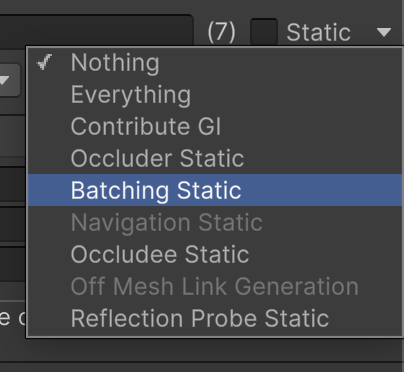
\includegraphics[width=0.5\textwidth]{immagini/cap2/unity_static_flag.png}
    \caption{Interfaccia di Unity nell'Inspector che mostra l'attivazione specifica del flag "Batching Static" per un oggetto statico.}
    \label{fig:unity_static_flag}
\end{figure}

Sebbene questo approccio aumenti l'utilizzo della memoria RAM, il vantaggio prestazionale è massimo: la CPU deve inviare un unico comando di disegno per l'intero gruppo, azzerando l'overhead di comunicazione per i singoli componenti.

\begin{lstlisting}[caption={Preprocessing logic for Static Batching.}]
// Initialization Phase (Build or Scene Load)
for each Material M in Scene:
    MeshList = FindStaticObjectsWith(M)
    CombinedMesh = new Mesh()
        
    for each Object in MeshList:
        // Transform vertices to world coordinates and merge
        WorldVertices = Object.mesh.TransformToWorldSpace()
        CombinedMesh.AddVertices(WorldVertices)
        
    // During Rendering Loop
    GPU.Draw(CombinedMesh, M)
\end{lstlisting}

\subsection{GPU Instancing} 

È la tecnica principale per renderizzare molteplici copie dello stesso modello geometrico utilizzando un set di dati condiviso \cite{AkenineRealTimeRendering}. A differenza del \textit{static batching}, questa tecnica non genera una nuova \textit{mesh} combinata; il motore invia alla GPU un'unica copia dei dati geometrici (vertici e indici) insieme a un \textit{array} di dati variabili, definiti \textit{per-instance data} (come matrici di trasformazione o variazioni di colore) \cite{UnityGPUInstancing}.

La GPU è quindi in grado di eseguire un ciclo di rendering interno estremamente efficiente, disegnando l'oggetto $N$ volte con una singola \textit{draw call}.

L'opzione deve essere esplicitamente abilitata nelle impostazioni del materiale.

\begin{figure}[H]
    \centering
    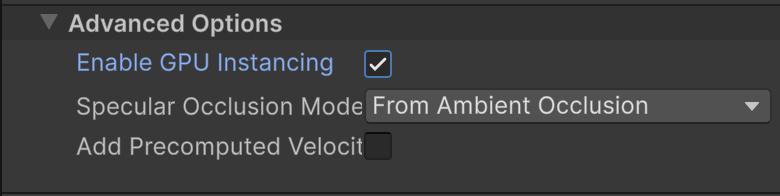
\includegraphics[width=0.7\textwidth]{immagini/cap2/gpu_instancing_flag.png}
    \caption{Abilitazione della spunta "Enable GPU Instancing" nelle "Advanced Options" di un materiale HDRP.}
    \label{fig:gpu_instancing_flag}
\end{figure}

    La logica di esecuzione a basso livello può essere schematizzata come segue:

\begin{lstlisting}[language=pseudo, caption={Algorithm for GPU Instancing execution.}, label={alg:gpu_instancing}]
// Prepare per-instance data arrays on CPU
TransformArray = [Pos1, Pos2, ... PosN]
PropertyArray  = [Color1, Color2, ... ColorN]

// Set the GPU state for the shared geometry
GPU.BindMesh(OriginalMesh)
GPU.BindMaterial(InstancedMaterial)

// Upload instance arrays to the GPU Constant Buffer
GPU.UploadToCBuffer(TransformArray, PropertyArray)

// Hardware-accelerated draw call for N instances
GPU.DrawInstanced(OriginalMesh, N)
\end{lstlisting}
    
\subsection{SRP Batcher} 
Rappresenta la tecnologia di punta per l'ottimizzazione in ambiente HDRP. A differenza delle tecniche di \textit{batching} tradizionali, che mirano esclusivamente a ridurre il numero assoluto di \textit{draw call}, l'SRP Batcher si focalizza sulla riduzione dei cambiamenti di stato tra una chiamata e l'altra. Questo avviene attraverso il raggruppamento di sequenze di comandi GPU di tipo \textit{bind} e \textit{draw} in quelli che vengono definiti \textit{SRP batch} \cite{UnitySRPBatcher}.
    
Il funzionamento del sistema si basa sulla persistenza dei dati dei materiali all'interno della memoria della GPU. L'SRP Batcher evita il caricamento ridondante dei dati se lo \textit{shader variant} rimane lo stesso.
    
\begin{figure}[H]
    \centering
    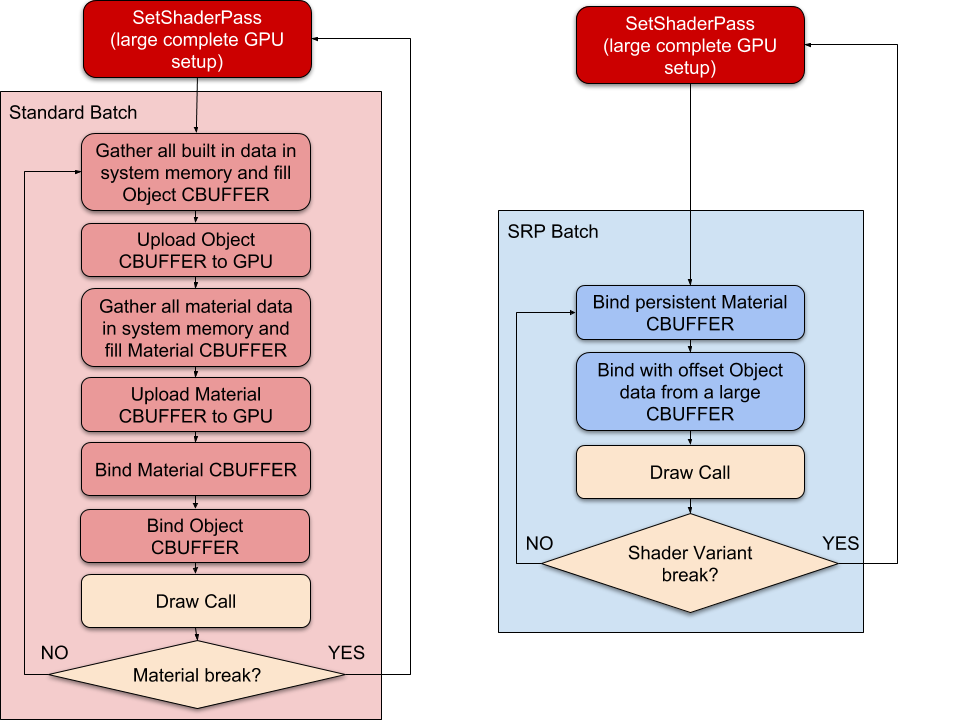
\includegraphics[width=0.85\textwidth]{immagini/cap2/SROShaderPass.png}
    \caption{Confronto tra il flusso di un batch standard e un SRP Batch.}
    \label{fig:srp_comparison}
\end{figure}
    
Dal punto di vista architettonico (Figura \ref{fig:srp_architecture}), quando il motore rileva un nuovo materiale, la CPU raccoglie tutte le proprietà e le lega alla GPU in appositi \textit{constant buffers} (CBUFFER). Se il contenuto del materiale non cambia, i dati persistono nella memoria video, rendendoli immediatamente pronti all'uso senza ulteriori interventi della CPU.
    
\begin{figure}[H]
    \centering
    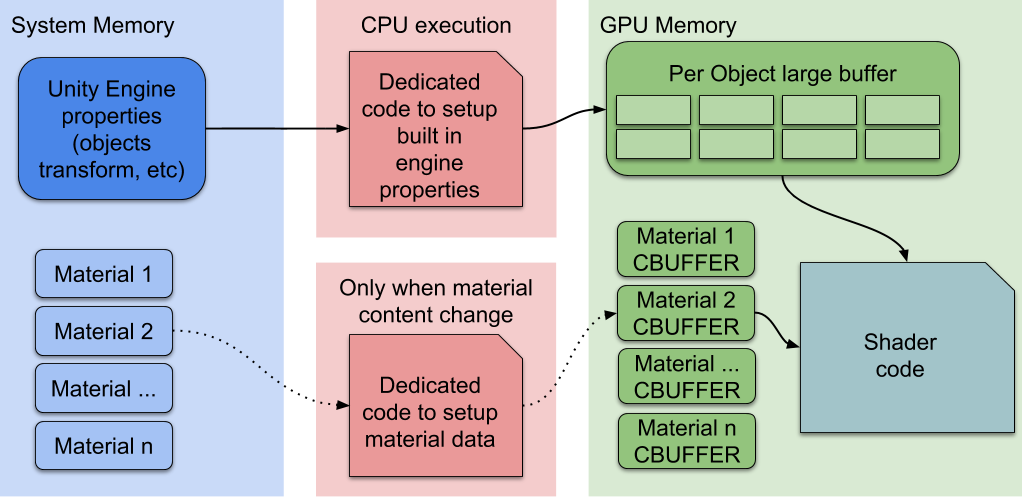
\includegraphics[width=0.9\textwidth]{immagini/cap2/SRP_Batcher_loop.png}
    \caption{Architettura della memoria nell'SRP Batcher.}
    \label{fig:srp_architecture}
\end{figure}
    
In questo scenario, il carico di lavoro del processore si riduce drasticamente, limitandosi alla gestione delle \textit{Unity Engine properties} (come le trasformazioni degli oggetti) all'interno di un unico grande buffer GPU (\textit{Per Object large buffer}).

\section{Shader: fondamenti teorici e linguaggio HLSL}

\subsection{Definizione di Shader}

Uno \textit{shader} è un programma, scritto in un linguaggio di alto livello, progettato per essere eseguito direttamente sulle unità di calcolo parallelo della GPU \cite{AkenineRealTimeRendering}. A differenza degli algoritmi eseguiti sulla CPU, che operano su flussi di dati generici, lo \textit{shader} ha il compito esclusivo di istruire il processore grafico su come trasformare i dati geometrici in informazioni visive (\textit{pixel}) \cite{HughesComputerGraphics}.

Il vantaggio fondamentale dello \textit{shader} risiede nell'architettura parallela della GPU: lo stesso codice viene eseguito contemporaneamente per migliaia di elementi diversi, garantendo una velocità di elaborazione che sarebbe impossibile da raggiungere con un'esecuzione sequenziale tradizionale.

\subsection{Classificazione degli Shader nella Pipeline Programmabile}

All'interno della moderna \textit{Graphics Pipeline}, le diverse fasi di elaborazione possono essere classificate in base alla loro flessibilità e necessità di implementazione da parte dello sviluppatore \cite{AkenineRealTimeRendering, ShirleyFundamentals}. Ogni blocco svolge una specifica funzione nel trasformare i dati in ingresso nell'immagine finale a schermo.

\begin{figure}[H]
    \centering
    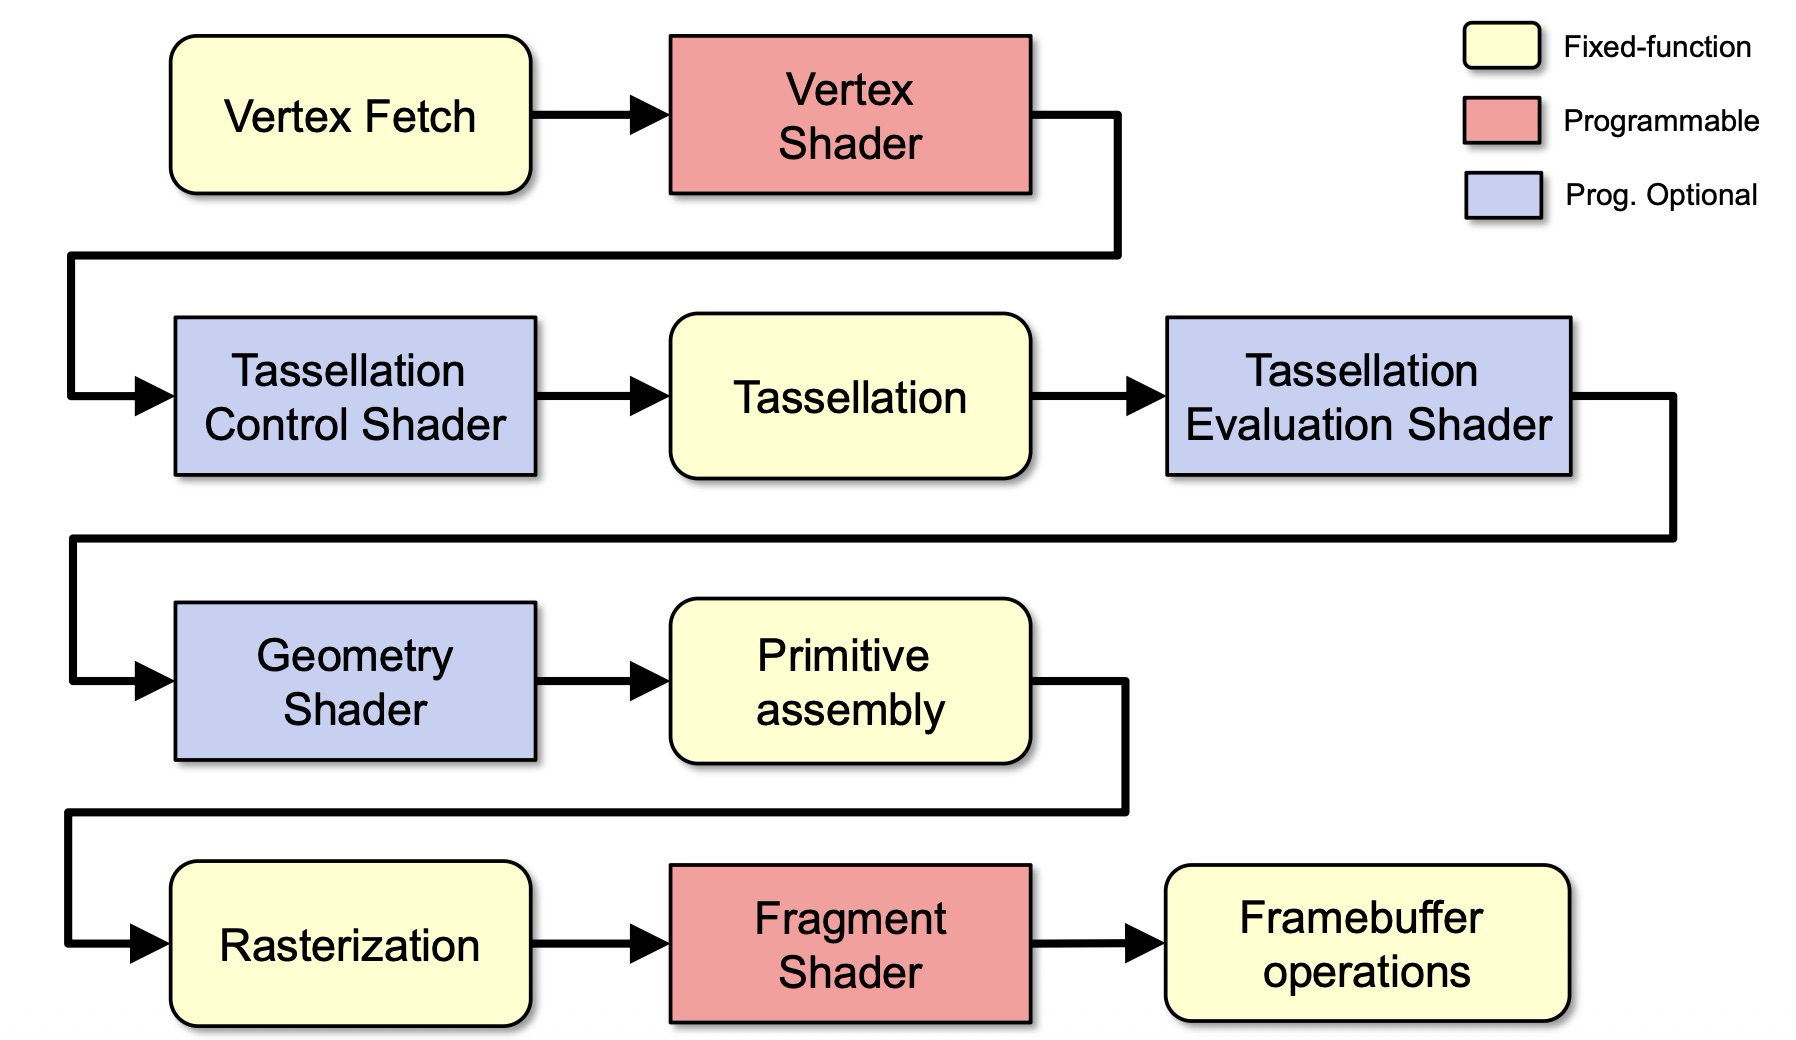
\includegraphics[width=\textwidth]{immagini/cap2/shaders_pipeline.png}
    \caption{Schema della Graphics Pipeline con distinzione tra blocchi fissi, programmabili e opzionali.}
    \label{fig:shaders_pipeline}
\end{figure}

Le macro-categorie che compongono l'architettura della pipeline sono:

\begin{itemize}
    \item \textbf{Blocchi Fissi:} Si tratta di fasi predefinite che utilizzano tecniche standard altamente ottimizzate a livello hardware. Non sono programmabili dall'utente e includono operazioni fondamentali come il \textit{Vertex Fetch}, la \textit{Tassellation} hardware e la \textit{Rasterization}.
    
    \item \textbf{Blocchi Programmabili:} Sono stadi che devono essere necessariamente implementati dallo sviluppatore attraverso la scrittura di appositi programmi chiamati \textit{Shader}. I due pilastri di questa categoria sono:
    \begin{itemize}
        \item \textbf{Vertex Shader:} Elabora ogni singolo vertice generandone gli attributi e applicando le trasformazioni geometriche necessarie per convertire le coordinate 3D nel sistema proiettivo.
        \item \textbf{Fragment Shader:} Riceve in input i frammenti generati dalla rasterizzazione e determina il colore effettivo di ogni pixel.
    \end{itemize}
    
    \item \textbf{Blocchi Programmabili Opzionali:} Rappresentano stadi aggiuntivi che vengono implementati solo se richiesto dalle specifiche necessità del rendering. Tra questi si distinguono:
    \begin{itemize}
        \item \textbf{Tassellation Control Shader (TCS):} Specifica il numero di vertici da generare per la suddivisone della primitiva.
        \item \textbf{Tassellation Evaluation Shader (TES):} Processa i nuovi vertici generati durante la fase di tassellazione.
        \item \textbf{Geometry Shader:} È in grado di modificare, eliminare o generare nuove primitive, cambiando potenzialmente la topologia della mesh (ad esempio, trasformando triangoli in linee).
    \end{itemize}
\end{itemize}

L'interazione tra questi blocchi permette un controllo granulare su ogni fase del rendering, partendo dal \textit{Vertex Fetch} dei dati (posizione 3D, vettori normali, colori e coordinate di \textit{texture}) fino alle operazioni finali sul \textit{Framebuffer}, dove i frammenti subiscono test di visibilità e profondità prima di essere scritti a schermo \cite{AkenineRealTimeRendering, HughesComputerGraphics}.
 % Contenuto: 2.1 HDRP, 2.2 Draw Call/Batching, 2.3 Shader teorico

\clearpage

% Capitolo 3: Profiling
\chapter{Analisi Iniziale delle Prestazioni}

L'ottimizzazione di un titolo in HDRP non può prescindere da una fase di misurazione rigorosa. Prima di applicare le tecniche di \textit{batching} e lo sviluppo di \textit{shader} ottimizzati, è necessario stabilire una metodologia di indagine che permetta di identificare con precisione i colli di bottiglia (\textit{bottleneck}) del sistema.

\section{Presentazione della scena di riferimento}

La scena selezionata per l'analisi delle prestazioni è denominata \textit{Chemical Plant}. Si tratta di un ambiente industriale di vaste dimensioni che alterna ampi spazi aperti a complessi interni strutturati su più livelli. Questa specifica ambientazione è stata scelta poiché integra diverse criticità tecniche che mettono sotto sforzo la \textit{High Definition Rendering Pipeline} (HDRP).

\subsection{Caratteristiche della Scena e Criticità Computazionali}

L'analisi si è focalizzata sui seguenti aspetti strutturali, rappresentativi delle sfide di ottimizzazione affrontate nel progetto:

\begin{itemize}
    \item \textbf{Densità di Asset Modulari:} La scena presenta una massiccia ripetizione di elementi geometrici complessi, quali tubature, valvole e strutture portanti metalliche. Se non gestiti correttamente tramite tecniche di \textit{batching}, tali oggetti generano un numero di \textit{draw call} insostenibile per la CPU.
    \item \textbf{Gestione degli Spazi Aperti:} Negli esterni, l'elevata distanza di rendering (\textit{draw distance}) obbliga il motore a processare un numero ingente di vertici, rendendo critico il sistema di \textit{culling} e la gestione dei \textit{Level of Detail} (LOD).
    \item \textbf{Illuminazione e Riflessioni:} Il contesto industriale richiede l'uso di numerosi \textit{point light} e \textit{spotlight} per simulare l'illuminazione artificiale dei macchinari. Inoltre, la presenza di materiali metallici e superfici con diversi gradi di \textit{smoothness} richiede calcoli intensivi per le riflessioni in tempo reale e le \textit{Shadow Maps}.
\end{itemize}

\begin{figure}[H]
    \centering
    \begin{minipage}{0.48\textwidth}
        \centering
        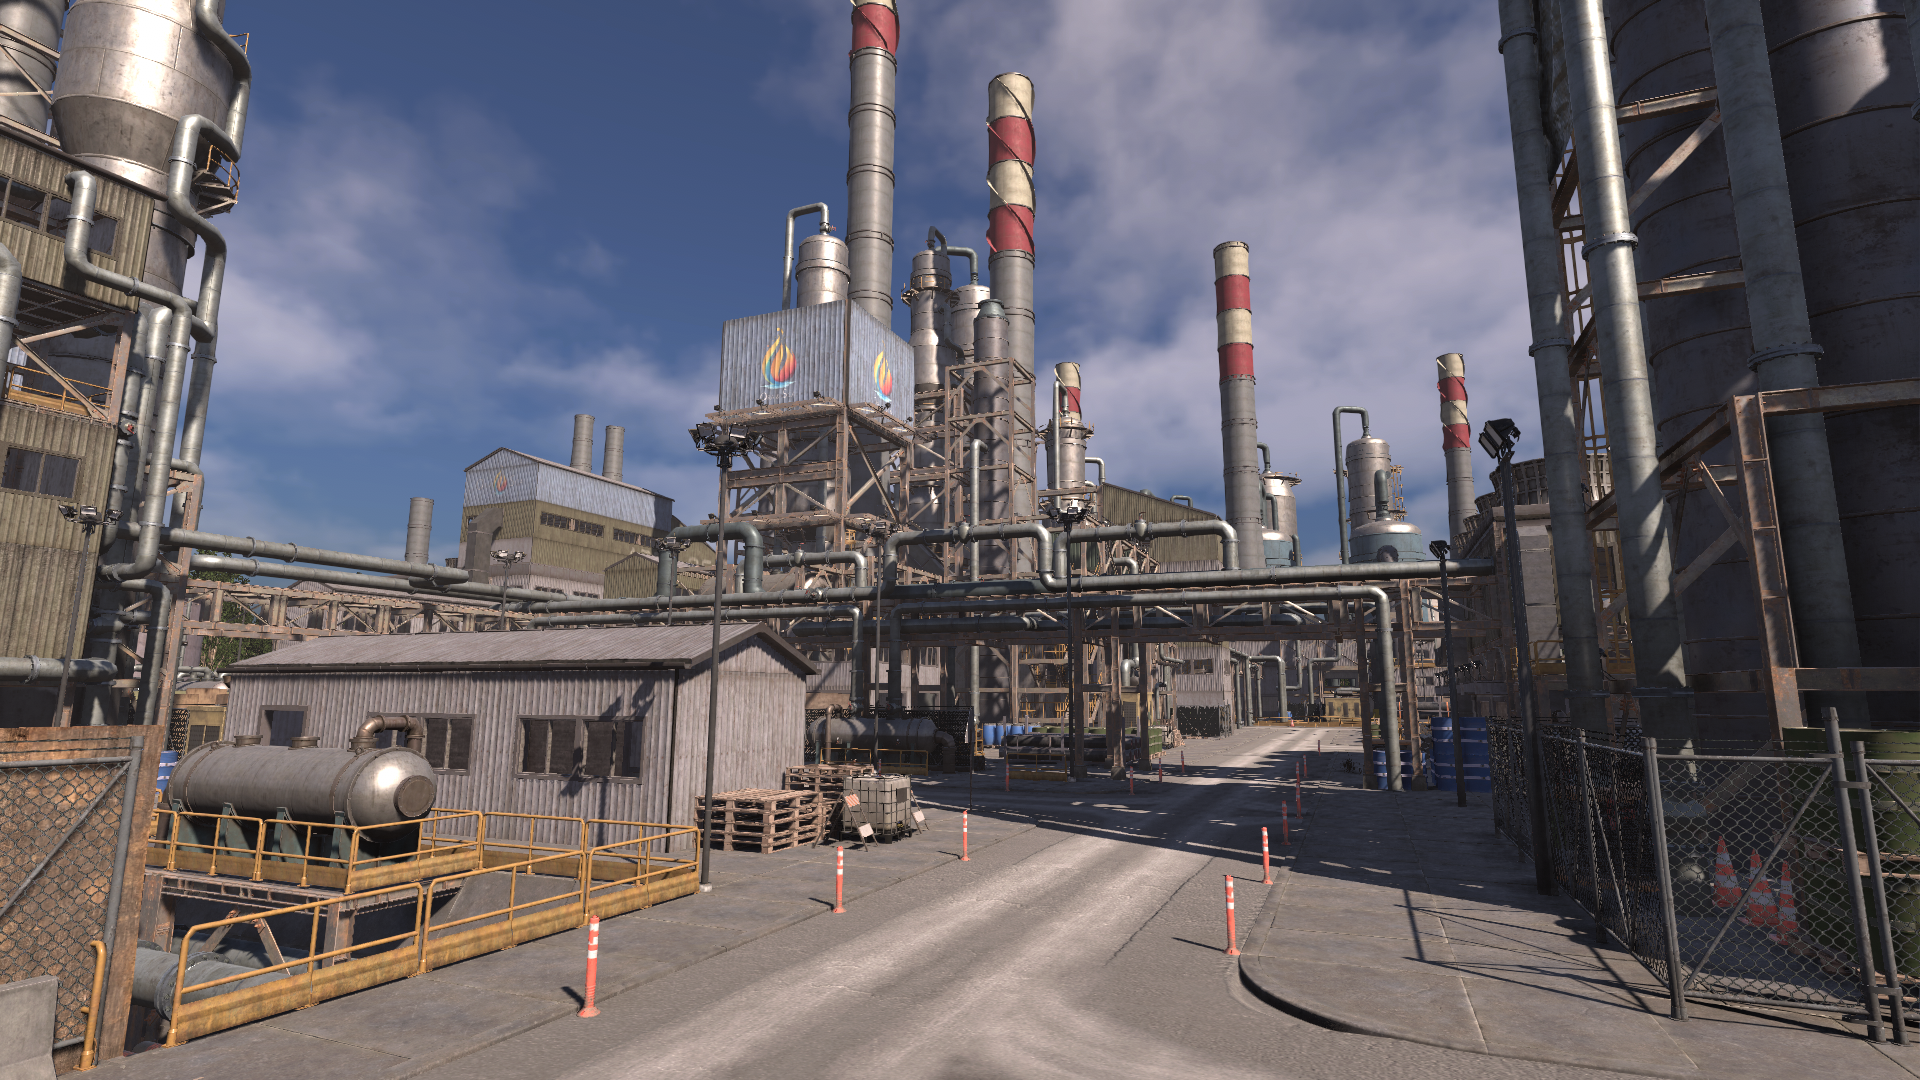
\includegraphics[width=\textwidth]{immagini/cap3/chemical_plant_outdoor.png}
        \caption*{\small (a) Outdoor Environment}
    \end{minipage}
    \hfill
    \begin{minipage}{0.48\textwidth}
        \centering
        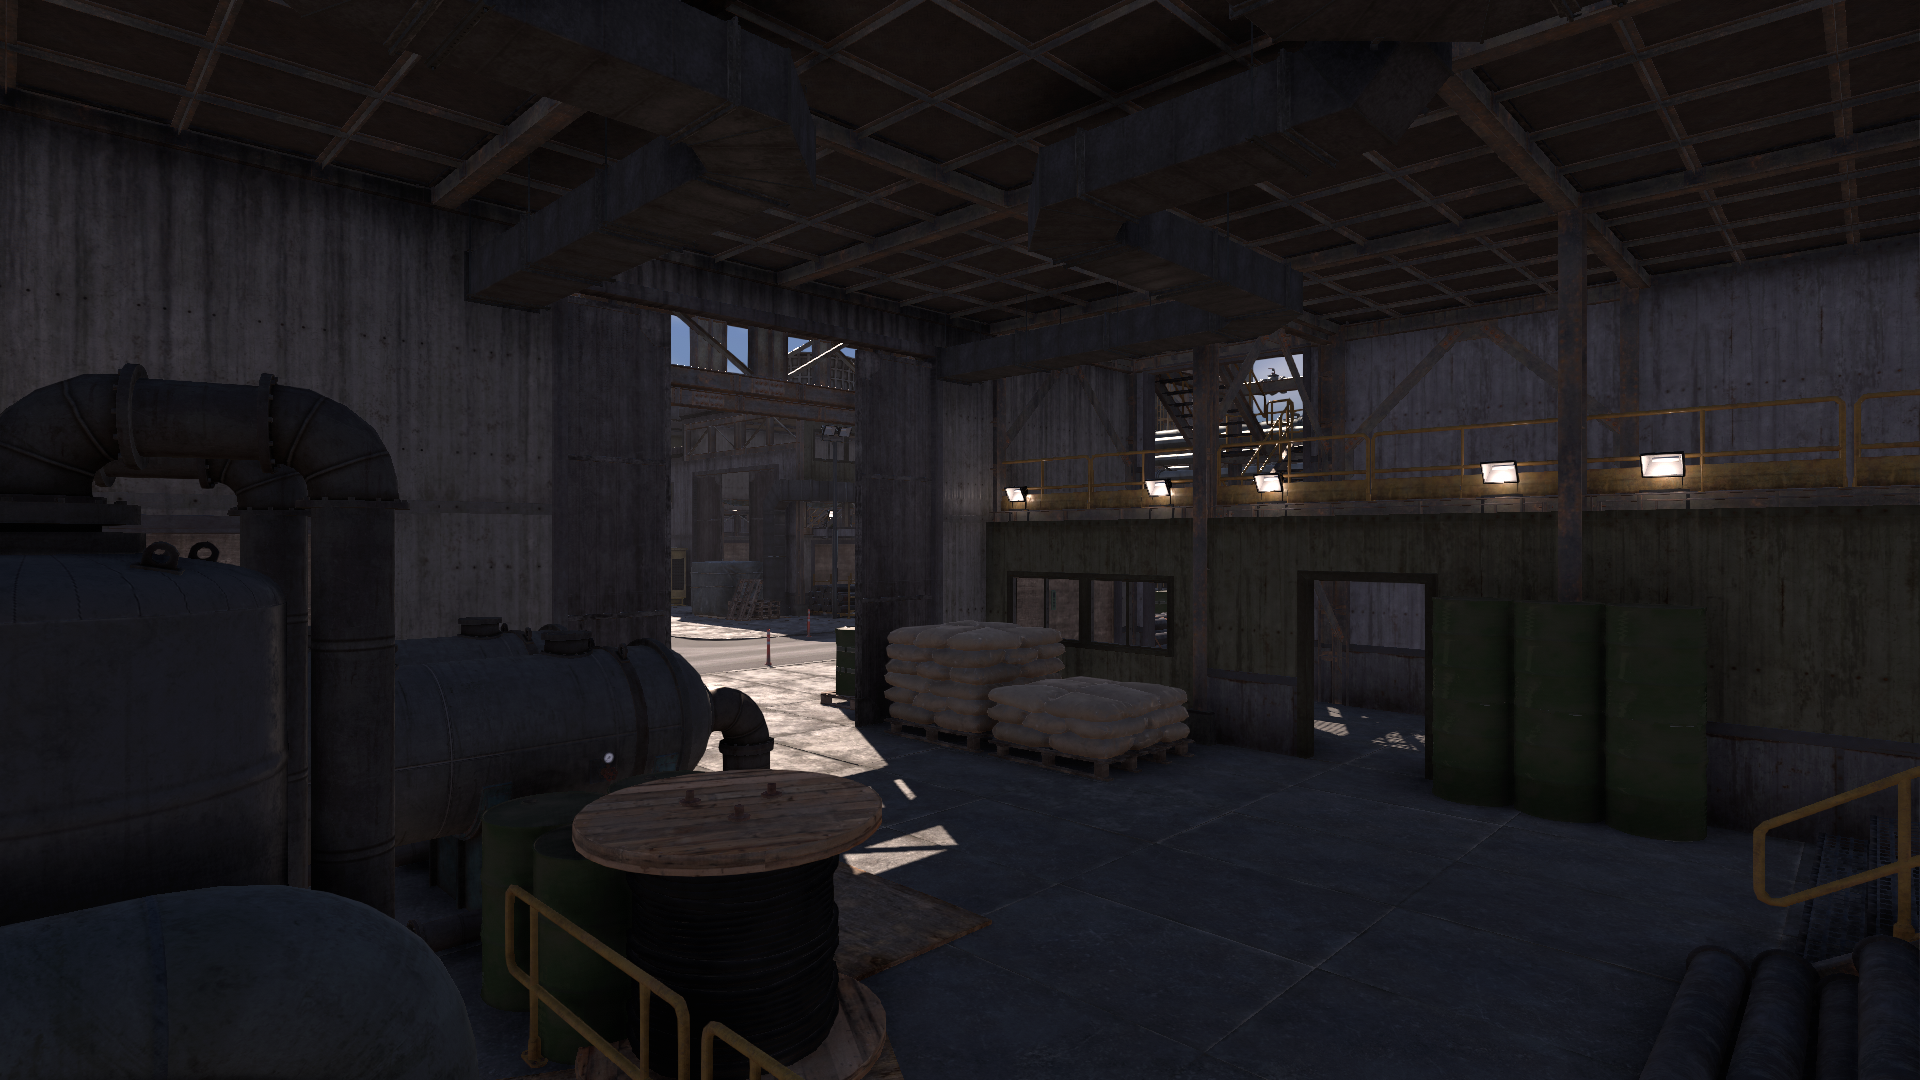
\includegraphics[width=\textwidth]{immagini/cap3/chemical_plant_indoor.png}
        \caption*{\small (b) Indoor Environment}
    \end{minipage}
    \caption{Dettagli della scena "Chemical Plant"}
    \label{fig:chemical_plant_details}
\end{figure}

\section{Strumenti di Profiling}

Per l'analisi quantitativa e qualitativa delle prestazioni di ARES, sono stati utilizzati i \textit{tool} ufficiali integrati nell'ecosistema Unity. Questi strumenti permettono di scindere il carico di lavoro del processore centrale (CPU) da quello della scheda grafica (GPU), identificando con precisione la natura dei colli di bottiglia.

\subsection{Unity Profiler}

L'Unity Profiler è lo strumento di analisi quantitativa fondamentale per monitorare l'allocazione delle risorse hardware in tempo reale. Esso permette di registrare le prestazioni del gioco durante l'esecuzione, fornendo un grafico temporale della durata di ogni singolo \textit{frame} suddiviso per moduli funzionali.

\subsubsection{Struttura e Moduli di Analisi}

L'interfaccia del Profiler è organizzata gerarchicamente per offrire diversi livelli di astrazione:

\begin{itemize}
    \item \textbf{Profiler Modules (Vista Macro):} Situata nella parte superiore, questa sezione mostra grafici a aree relativi a diverse categorie di consumo. Per l'ottimizzazione di ARES, il modulo \textit{Rendering} risulta critico, in quanto riporta il numero di \textit{Draw Calls}, \textit{SetPass Calls} e il tempo totale speso dalla CPU per istruire la pipeline grafica.
    \item \textbf{Timeline View (Vista Micro):} Posizionata nella parte inferiore, questa vista visualizza l'esecuzione parallela dei diversi \textit{thread} del motore. È stata utilizzata per analizzare la sincronizzazione tra il \textbf{Main Thread} e il \textbf{Render Thread}.
\end{itemize}

\begin{figure}[H]
    \centering
    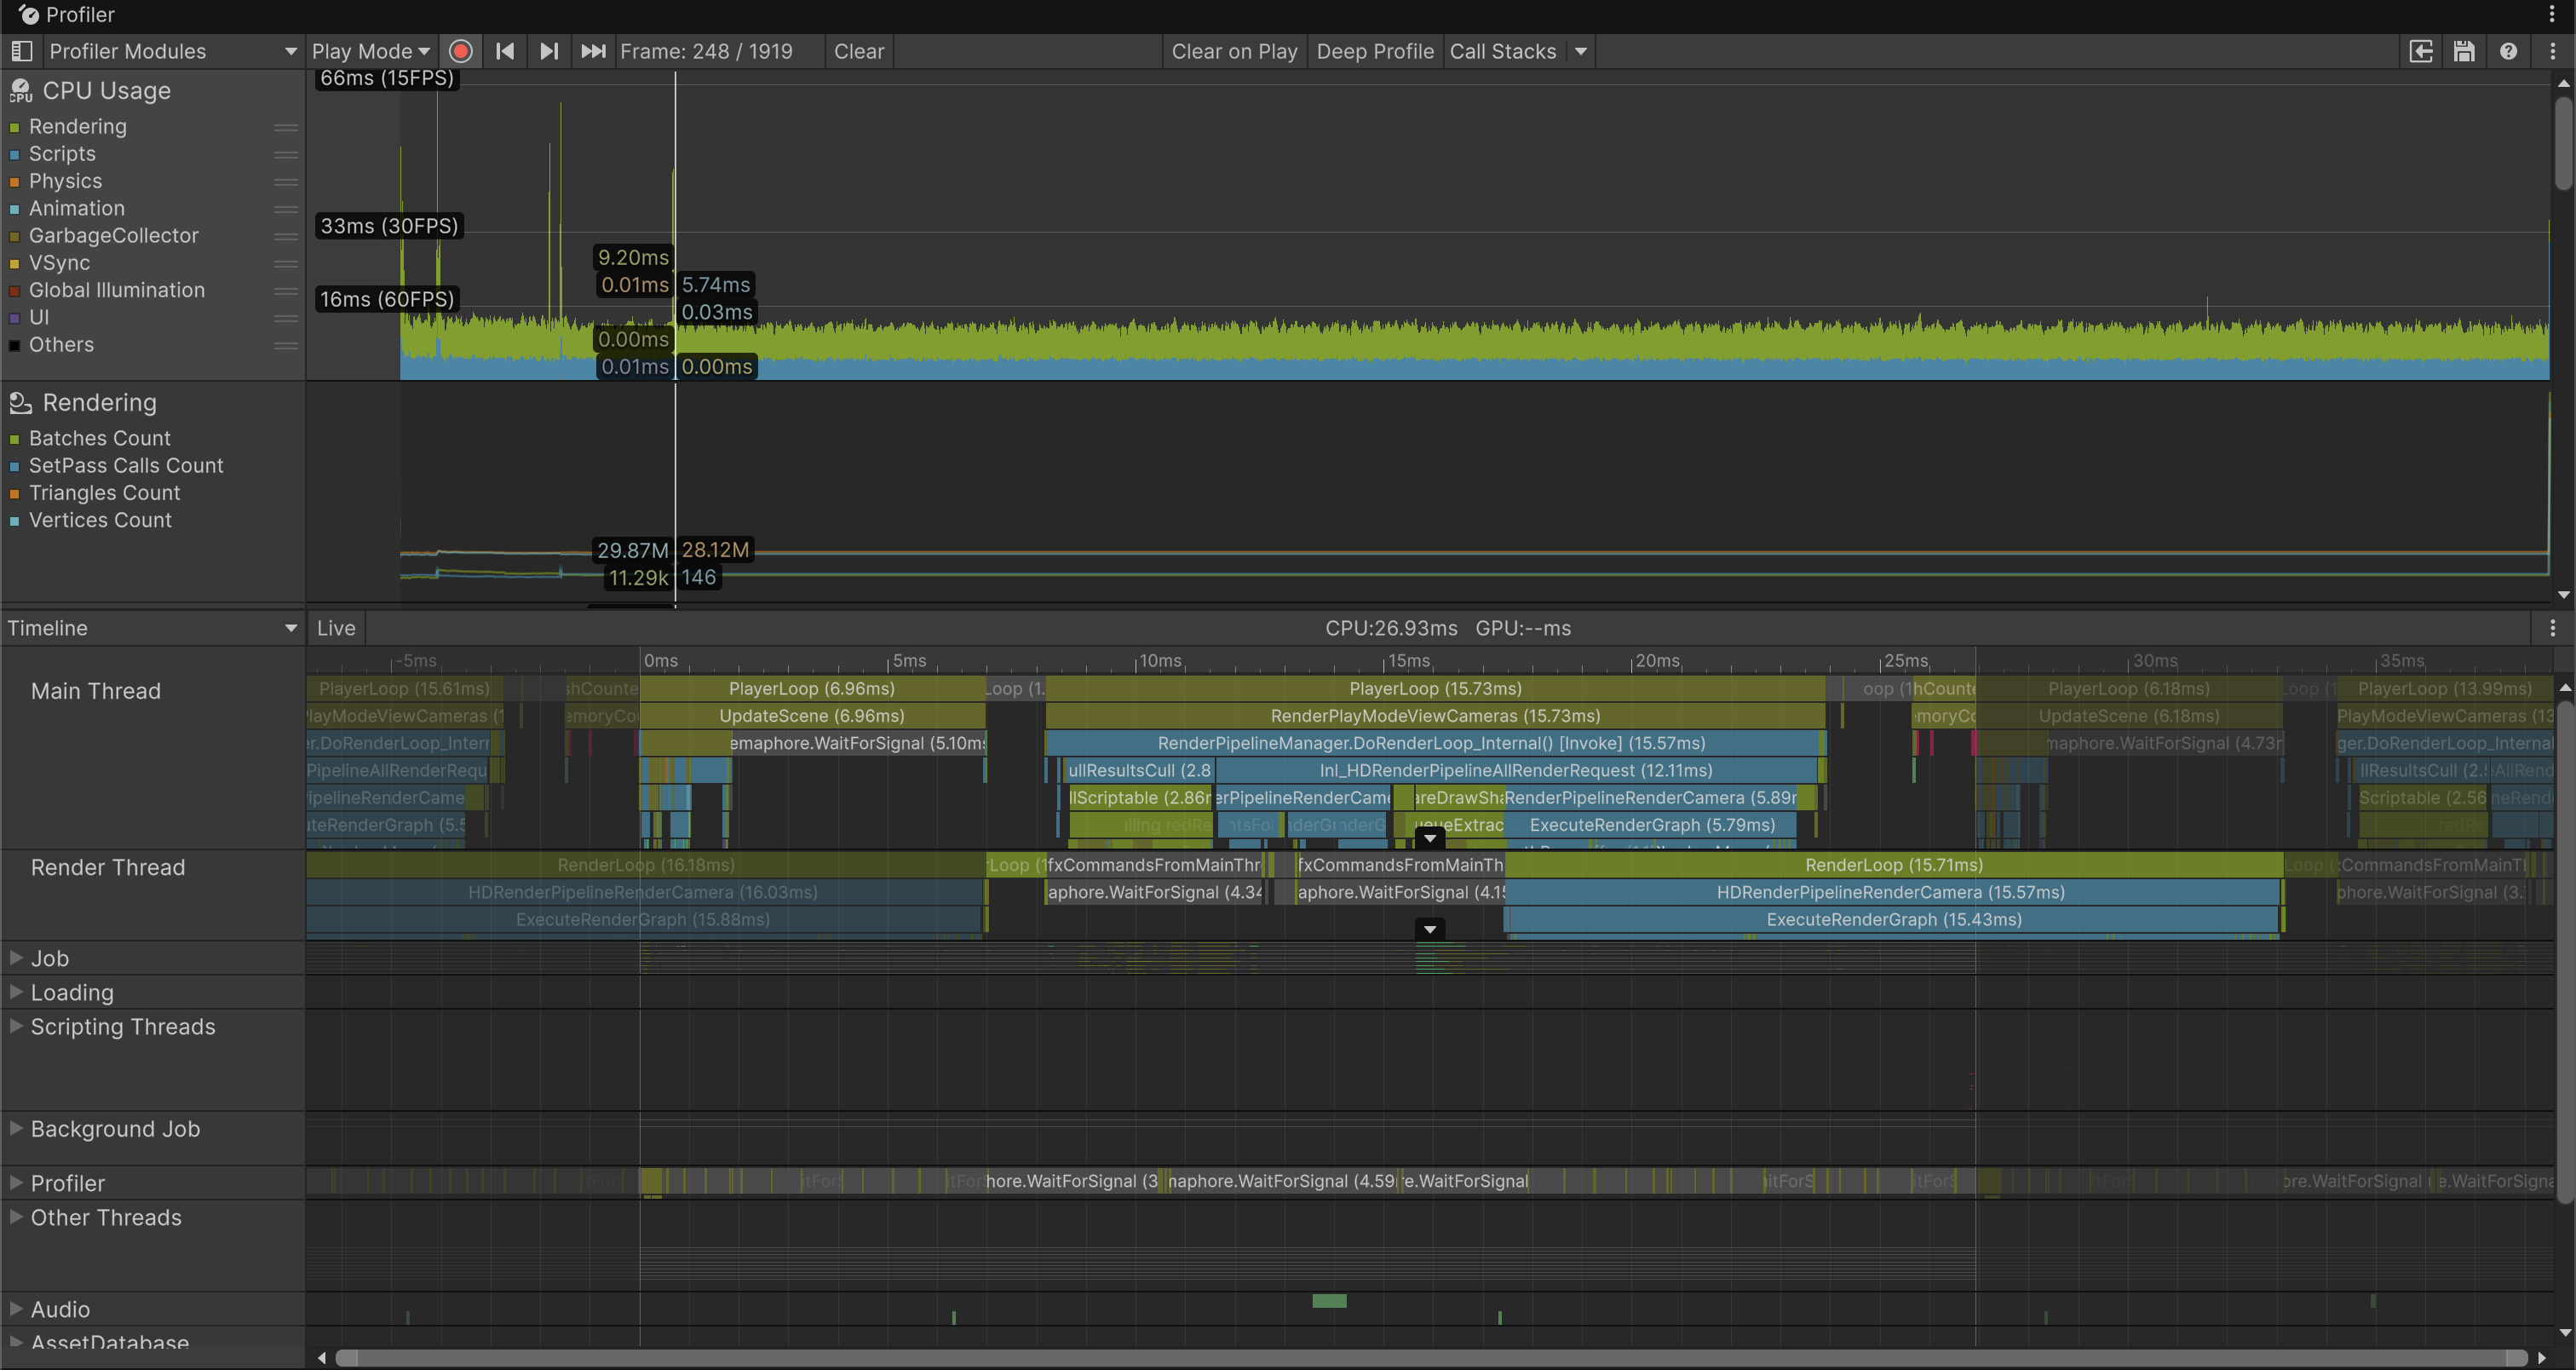
\includegraphics[width=\textwidth]{immagini/cap3/unity_profiler_structure.png}
    \caption{Analisi dettagliata tramite Unity Profiler in modalità Timeline. Nella sezione inferiore è possibile osservare la distribuzione del carico di lavoro tra Main Thread e Render Thread, identificando i tempi di esecuzione delle funzioni di rendering della HDRP.}
    \label{fig:profiler_structure}
\end{figure}

\subsubsection{Metriche Critiche per l'Ottimizzazione}

Prima di procedere con la fase sperimentale, è fondamentale definire le metriche prestazionali che fungeranno da indicatori chiave per valutare l'efficacia degli interventi di ottimizzazione. Queste grandezze, monitorate attraverso i moduli del Profiler, permettono di mappare il carico di lavoro tra i diversi componenti hardware.

Le metriche selezionate per lo studio della scena \textit{Chemical Plant} sono:

\begin{itemize}
    \item \textbf{Batches e SetPass Calls:} I \textit{Batches} indicano il numero di pacchetti di geometria inviati alla GPU per il disegno. Le \textit{SetPass Calls} rappresentano invece quante volte la GPU deve cambiare il proprio stato interno per elaborare un nuovo materiale o shader. Una riduzione di questi valori indica una migliore aggregazione dei dati e un minor carico sulla CPU.
    
    \item \textbf{Frame Time (ms):} Rappresenta il tempo totale impiegato dal sistema per completare tutte le fasi della pipeline. È la metrica principale per determinare la fluidità dell'applicazione, dove tempi inferiori corrispondono a un \textit{frame rate} (FPS) più elevato.
    
    \item \textbf{Triangles e Vertices Count:} Indicano la densità geometrica complessiva processata nel \textit{Vertex Shader}. Monitorare questi valori permette di verificare l'impatto visivo e prestazionale delle tecniche di semplificazione della mesh.
    
    \item \textbf{Gfx.Wait Commands:} Questi marcatori, visibili nella \textit{Timeline View}, indicano i tempi di inattività in cui un thread (Main o Render) rimane in attesa del completamento di un'operazione da parte di un altro componente. L'analisi di questi tempi è essenziale per identificare se il collo di bottiglia risiede nell'elaborazione dei dati (CPU) o nel disegno effettivo dei pixel (GPU).
\end{itemize}

\subsection{Frame Debugger}

Il \textbf{Frame Debugger} è lo strumento fondamentale per l'analisi analitica di ogni singolo fotogramma prodotto dalla pipeline HDRP. A differenza del Profiler, che monitora l'andamento temporale, il Frame Debugger permette di "congelare" il rendering e ispezionare sequenzialmente tutti i comandi inviati dalla CPU alla GPU (\textit{Draw Calls}).

L'utilizzo di questo strumento nella scena \textit{Chemical Plant} ha permesso di:
\begin{itemize}
    \item \textbf{Analizzare la gerarchia del rendering:} Osservare l'ordine cronologico con cui gli oggetti vengono processati, dalla fase di \textit{Depth Prepass} fino al \textit{Post-processing}.
    \item \textbf{Diagnosticare le interruzioni dei batch:} Identificare le cause specifiche che impediscono al motore di raggruppare più oggetti in un'unica operazione di disegno.
    \item \textbf{Verificare gli stati della pipeline:} Controllare quali shader sono attivi per ogni oggetto e come i dati fluiscono attraverso i blocchi programmabili descritti precedentemente.
\end{itemize}

\begin{figure}[H]
    \centering
    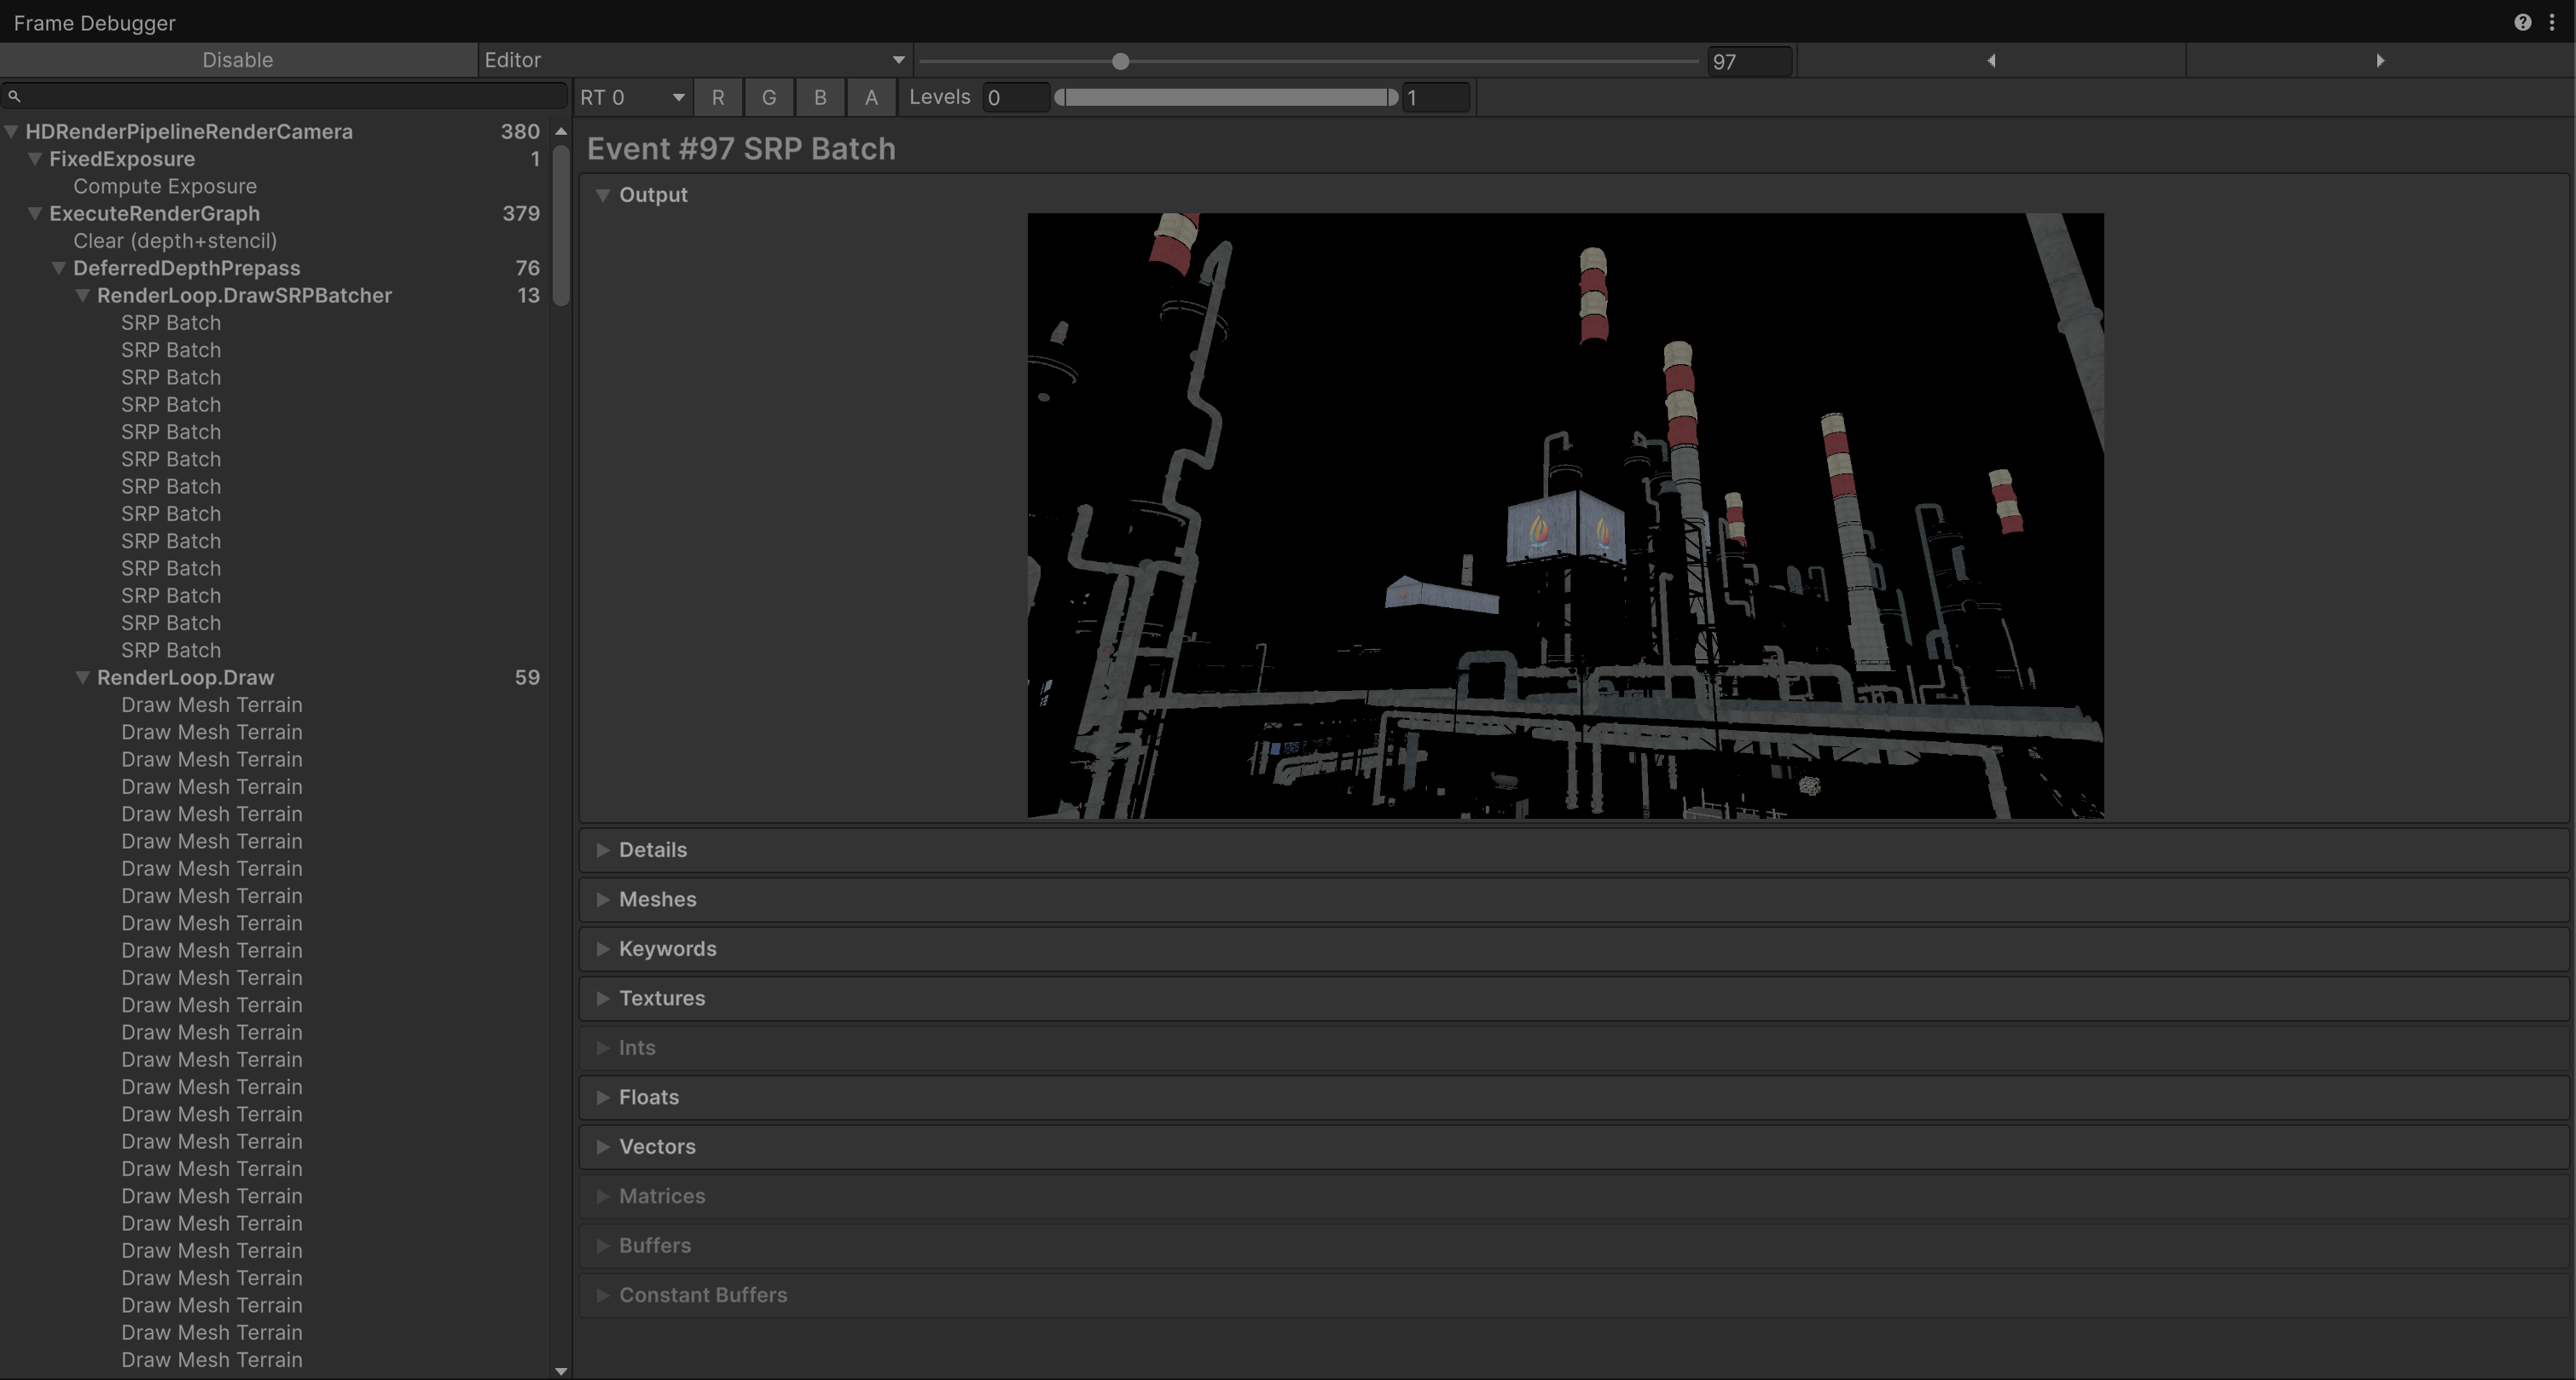
\includegraphics[width=\textwidth]{immagini/cap3/frame_debugger.png}
    \caption{Analisi della scena Chemical Plant tramite Frame Debugger. È possibile osservare la suddivisione delle operazioni di rendering, con particolare evidenza sulle numerose istanze di "Draw Mesh" che non vengono ancora aggregate efficacemente, contribuendo all'elevato numero di draw call totali.}
    \label{fig:frame_debugger}
\end{figure}

\section{Rilevazione della Baseline}

Il processo di analisi ha inizio con la determinazione della \textit{baseline} prestazionale, ovvero la misurazione dello stato del progetto prima di ogni intervento correttivo. Per garantire l'oggettività e la riproducibilità dei dati, la raccolta è stata effettuata attraverso l'impiego di una cinematica fissa. Questo approccio permette di analizzare carichi computazionali identici in ogni sessione di test, rendendo i dati confrontabili tra le diverse iterazioni del processo di ottimizzazione.

\subsection{Setup Sperimentale e Condizioni di Test}

Le rilevazioni sono state condotte su un'unica configurazione hardware di riferimento per isolare le variabili prestazionali legate esclusivamente al motore grafico. Il sistema utilizzato è un \textbf{MacBook Pro} equipaggiato con chip \textbf{Apple M2 Pro}.

Al fine di sottoporre la pipeline HDRP a uno stress test significativo, le impostazioni del motore sono state configurate come segue:
\begin{itemize}
    \item \textbf{Risoluzione:} 1920x1080 (Full HD).
    \item \textbf{Preset di Qualità:} Ultra (impostazioni massime previste dalla HDRP).
    \item \textbf{Metodologia:} Profiling in tempo reale durante l'esecuzione della cinematica fissa.
\end{itemize}

\subsection{Analisi Quantitativa delle Metriche di Rendering}

I dati raccolti evidenziano uno stato di forte inefficienza della pipeline, con valori che superano le soglie ottimali per il target hardware individuato. Di seguito vengono analizzate le metriche fondamentali registrate nei punti di maggiore criticità del percorso.

\subsubsection{Geometria ed Efficienza dei Batch}

L'analisi combinata del carico geometrico e della gestione delle chiamate al disegno rivela le principali criticità che gravano sia sulla CPU che sulla GPU:

\begin{itemize}
    \item \textbf{Complessità Geometrica:} La scena presenta un volume di \textbf{28.13 M di triangoli} e \textbf{29.85 M di vertici}. Tale densità poligonale risulta eccessiva per le reali necessità visive, saturando la pipeline già nella fase di \textit{Vertex Shading} e appesantendo inutilmente la fase di rasterizzazione.
    \item \textbf{Frammentazione delle Draw Calls (11.20 k Batches):} Questo valore rappresenta il principale collo di bottiglia del sistema. Un numero di batch così elevato genera un \textit{overhead} insostenibile per il \textit{Render Thread}, indicando una comunicazione inefficiente tra il processore e la scheda video.
    \item \textbf{Cambi di Stato (146 SetPass Calls):} Sebbene meno critico del batch count, il numero di \textit{SetPass Calls} conferma una mancata standardizzazione dei materiali e degli shader, che interrompe frequentemente la sequenza di invio dei comandi alla GPU.
\end{itemize}

\begin{figure}[H]
    \centering
    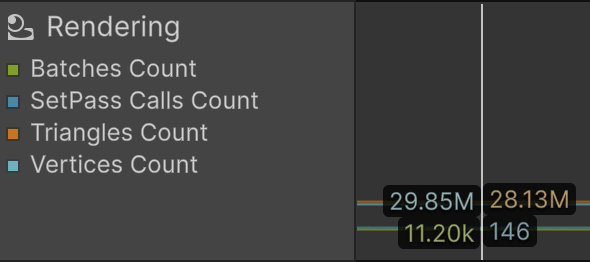
\includegraphics[width=0.9\textwidth]{immagini/cap3/profiler_rendering_baseline.png}
    \caption{Rilevazione dei parametri critici tramite Unity Profiler: si noti l'impatto combinato dell'elevata densità poligonale e degli 11.20k batches sul tempo di frame.}
    \label{fig:profiler_metrics_baseline}
\end{figure}

\subsubsection{Profiling della Timeline}

Per isolare con precisione la causa della bassa frequenza di aggiornamento, è stata effettuata un'analisi granulare del singolo fotogramma attraverso la \textit{Timeline View} del Profiler. Lo \textit{screenshot} riportato in Figura \ref{fig:profiler_timeline_frame} illustra la sequenza temporale delle operazioni eseguite dai thread principali durante un frame rappresentativo della baseline, con un tempo di calcolo complessivo di $32.59\text{ ms}$ (corrispondenti a circa $30\text{ FPS}$).

\begin{figure}[H]
    \centering
    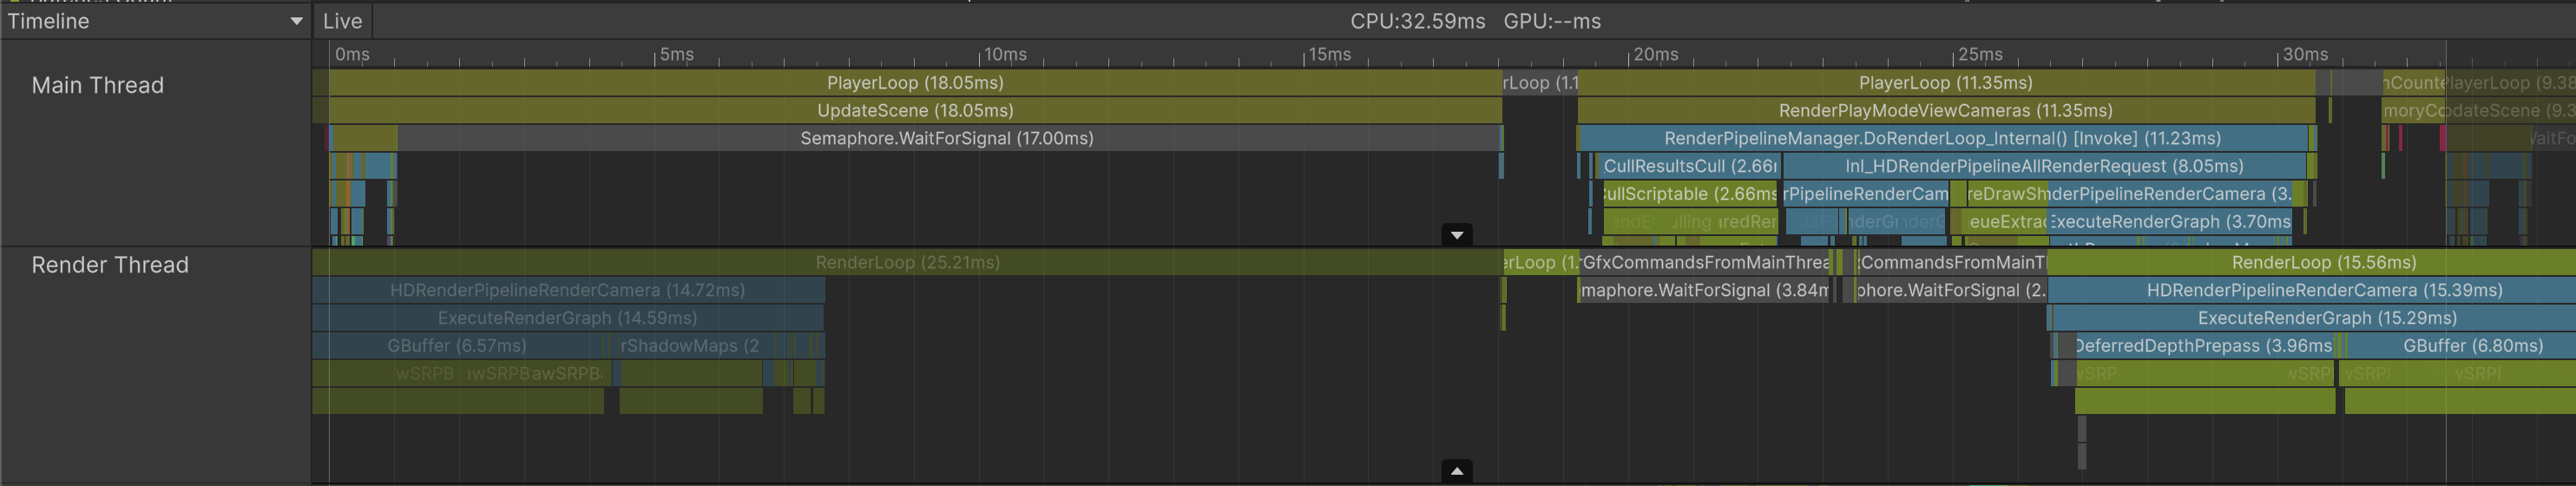
\includegraphics[width=\textwidth]{immagini/cap3/profiler_timeline_baseline.png}
    \caption{Dettaglio della Timeline View: analisi della sincronizzazione tra Main Thread e Render Thread in un singolo fotogramma.}
    \label{fig:profiler_timeline_frame}
\end{figure}

L'ispezione della Timeline permette di scomporre il lavoro del motore e identificare i seguenti problemi strutturali:

\begin{itemize}
    \item \textbf{Stallo del Main Thread (Semaphore):} L'evidenza più significativa è rappresentata dal blocco denominato \textit{Semaphore.WaitForSignal}, che occupa ben $17.00\text{ ms}$ del tempo totale. Sebbene il processore abbia completato la logica di gioco (\textit{PlayerLoop}), esso rimane inattivo in attesa che il \textit{Render Thread} termini l'elaborazione del fotogramma precedente. Questo fenomeno indica che il sistema è \textbf{Render-Thread bound}.
    
    \item \textbf{Sovraccarico del Render Thread:} Il \textit{Render Thread} mostra un \textit{RenderLoop} estremamente esteso ($25.21\text{ ms}$). Al suo interno, la funzione \textit{ExecuteRenderGraph} è rallentata dalla mole spropositata di istruzioni prodotte dagli oltre 11.000 batch. Il thread di rendering agisce come un collo di bottiglia: dovendo "impacchettare" migliaia di piccole chiamate singole per la GPU, non riesce a liberare il \textit{Main Thread} in tempi utili per il fotogramma successivo.
    
    \item \textbf{Culling:} All'interno del \textit{Main Thread}, la fase di \textit{CullResults.Cull} ($2.86\text{ ms}$) risulta proporzionalmente onerosa. Unity deve testare la visibilità di migliaia di oggetti individuali.
    
    \item \textbf{Passaggi HDRP (G-Buffer e Shadow Maps):} Nella parte terminale della sequenza, si osservano i tempi dedicati al \textit{Deferred Depth Prepass} e alla scrittura del \textit{G-Buffer}. L'estensione di questi blocchi conferma che l'alta densità poligonale (28M di triangoli) e la gestione delle ombre proiettate contribuiscono ulteriormente a dilatare il tempo di esecuzione del comando di disegno finale.
\end{itemize}

In sintesi, l'analisi della baseline dimostra che il vero problema non risiede nella potenza della scheda video, ma nella comunicazione tra i componenti del motore. Il sistema impiega troppo tempo nella fase di organizzazione dei dati: il \textbf{Render Thread} è letteralmente sommerso da migliaia di istruzioni individuali e non riesce a "dire" alla GPU cosa disegnare in tempi rapidi. 

Questo genera un effetto a catena che blocca l'intero processo, costringendo il processore a lunghe attese inutili. Risulta quindi evidente che la priorità assoluta per l'ottimizzazione sia l'implementazione di un \textbf{batching} più efficiente, capace di raggruppare questi migliaia di piccoli comandi in pochi blocchi più grandi e gestibili. % Contenuto: 3.1 Scena rif, 3.2 Tool Profiling, 3.3 Baseline

\clearpage

% Capitolo 4: Ottimizzazione pratica
\chapter{Ottimizzazione}
\section{Riduzione delle Draw Call}
[cite_start]Applicazione di strategie di pre-processing e raggruppamento per ridurre il carico sulla CPU. [cite: 79]

\section{Sviluppo di Shader personalizzati}
[cite_start]Dettagli sull'ottimizzazione degli shader per Ares per ridurre le chiamate al sistema e migliorare l'efficienza matematica. [cite: 79]

\section{Gestione dell'illuminazione: Real-Time vs Baking}
[cite_start]Confronto tra le tecniche di illuminazione studiate durante lo stage. [cite: 79] % Contenuto: 4.1 Riduzione Draw Call, 4.2 Shader custom, 4.3 Lighting/Baking

\clearpage

% Capitolo 5: Risultati
\chapter{Valutazione dei Risultati}
\section{Analisi comparativa}
[cite_start]Confronto tra i dati della baseline (Capitolo 3) e i risultati ottenuti post-ottimizzazione, con l'ausilio di grafici e tabelle prestazionali. [cite: 79, 80] % Contenuto: 5.1 Analisi comparativa

\clearpage

% Conclusioni
\addcontentsline{toc}{chapter}{Conclusioni} 
\chapter*{Conclusioni}
[cite_start]Sintesi dei risultati raggiunti durante le 300 ore di stage e possibili sviluppi futuri per il rendering di Ares. [cite: 57] % Crea il file conclusioni.tex

\clearpage

\printbibliography
\addcontentsline{toc}{chapter}{Bibliografia}

\end{document}